\documentclass[11pt,a4paper]{report}
\usepackage[ngerman]{babel} % deutsch und deutsche Rechtschreibung
\usepackage[utf8]{inputenc} % Unicode Text 
\usepackage[T1]{fontenc} % Umlaute und deutsches Trennen
\usepackage{textcomp} % Sonderzeichen wie Euro, Copyright, etc.
\usepackage[hyphens]{url} % Hyperlinks, eMail-Adressen, Pfadangaben
\usepackage{amssymb} % mathmatische Symbole
\usepackage{microtype} % reguliert Abstände zwischen Buchenstaben
\usepackage{graphicx} % wir wollen Bilder einfügen
\usepackage{float} % Umgebung die sich automatisch im Dokument an passenden Positionen bewegen (floaten)
\usepackage{emptypage} % Wirklich leer bei leeren Seiten
\usepackage{paralist} % Spezielle Aufzählungstypen wie z.B. begin{compactenum}[a)] https://de.wikibooks.org/wiki/LaTeX-W%C3%B6rterbuch:_Aufz%C3%A4hlung
\usepackage[german=quotes]{csquotes} % Für deutsche Anführungsstriche
\usepackage{hyperref} % macht ToC und alle internen Lonks klickbar (für leichtere Navigation)
\hypersetup{
    colorlinks,
    citecolor=black,
    filecolor=black,
    linkcolor=black,
    urlcolor=black
}

\usepackage{listings} % schöne Quellcode-Listings
% ein paar Einstellungen für akzeptable Listings
\lstset{basicstyle=\ttfamily, columns=[l]flexible, mathescape=true, showstringspaces=false, numbers=left, numberstyle=\tiny}
\lstset{language=C++} % Set your language (you can change the language for each code-block optionally)
% more information about listings: https://en.wikibooks.org/wiki/LaTeX/Source_Code_Listings

% Spezialpakete
\usepackage{epigraph} % Zum Positionieren von Bemerkungen links, rechts, oben und unten vom Text
\setlength{\epigraphrule}{0pt} % kein Trennstrich

% Seitenlayout
\usepackage[paper=a4paper,width=14cm,left=35mm,height=22cm]{geometry}
\usepackage{setspace}
\linespread{1.15}
\setlength{\parskip}{0.5em}
\setlength{\parindent}{0em} % im Deutschen Einrückung nicht üblich, leider

\newcommand{\phv}{\fontfamily{phv}\fontseries{m}\fontsize{9}{11}\selectfont}
\usepackage{fancyhdr} % ermöglicht schickere Header und Footer
\pagestyle{fancy}
\renewcommand{\chaptermark}[1]{\markboth{#1}{}}
\fancyhead[L]{\phv \leftmark}
\fancyhead[RE,LO]{\phv \nouppercase{\leftmark}}
\fancyhead[LE,RO]{\phv \thepage}
% Unten besser auf alles Verzichten
%\fancyfoot[L]{\textsf{\small \kurztitel}}
\fancyfoot[C]{\ } % keine Seitenzahl unten
%\fancyfoot[R]{\textsf{\small Medieninformatik}}

% Quellen aufteilen z.B. in Online-Quellen und Literaturverzeichnis
\usepackage{bibtopic} 

% Config 1: Times New Roman, gewohnter Font, ok tt und serifenlos
%\usepackage{mathptmx} 
%\usepackage[scaled=.95]{helvet}
%\usepackage{courier}

% Config 2: Palatino mit guten Fonts für tt und serifenlos
\usepackage{mathpazo} % Palatino, mal was anderes
\usepackage[scaled=.95]{helvet}
\usepackage{palatino}

% Config 3: New Century Schoolbook sieht auch nett aus (macht auch tt und serifenlos)
%\usepackage{newcent}

% Mehr Informationen zu Fonts: https://de.sharelatex.com/learn/Font_typefaces


% Zum Zeigen von Fehlern
\usepackage{soulutf8}
\newcommand*\falsch{\st}

% damit wir nicht so viel tippen müssen, nur für Demo 
%\usepackage{blindtext} 

% Float-Objekte sollen die (Sub)Section nicht verlassen in der sie eingefügt worden sind
\usepackage[section]{placeins}

% Für den Befehl \FloatBarrier - Damit kann man Grenzen für Float-Objekte erstellen, die sie nicht verlassen dürfen.
\usepackage{placeins}

% Für farbige Schriften 
\usepackage{color}

\definecolor{mygreen}{rgb}{0,0.6,0}
\definecolor{mygray}{rgb}{0.5,0.5,0.5}
\definecolor{mymauve}{rgb}{0.58,0,0.82}

\lstset{ %
  backgroundcolor=\color{white},   % choose the background color; you must add \usepackage{color} or \usepackage{xcolor}
  basicstyle=\footnotesize\ttfamily,        % the size of the fonts that are used for the code
  breakatwhitespace=false,         % sets if automatic breaks should only happen at whitespace
  breaklines=true,                 % sets automatic line breaking
  captionpos=b,                    % sets the caption-position to bottom
  commentstyle=\color{mygreen},    % comment style
  deletekeywords={...},            % if you want to delete keywords from the given language
	otherkeywords={...},           % if you want to add more keywords to the set
  escapeinside={\%*}{*)},          % if you want to add LaTeX within your code
  extendedchars=true,              % lets you use non-ASCII characters; for 8-bits encodings only, does not work with UTF-8
  frame=none,	                   % adds a frame around the code
  keepspaces=true,                 % keeps spaces in text, useful for keeping indentation of code (possibly needs columns=flexible)
  keywordstyle=\color{blue},       % keyword style
  language=C++,                    % the language of the code
  numbers=left,                    % where to put the line-numbers; possible values are (none, left, right)
  numbersep=10pt,                   % how far the line-numbers are from the code
  numberstyle=\footnotesize, % the style that is used for the line-numbers
  rulecolor=\color{black},         % if not set, the frame-color may be changed on line-breaks within not-black text (e.g. comments (green here))
  showtabs=false,                  % show tabs within strings adding particular underscores
  stepnumber=1,                    % the step between two line-numbers. If it's 1, each line will be numbered
  tabsize=1,	                   % sets default tabsize to 2 spaces
}

%\lstdefinestyle{foo}{
%  moredelim=[is][\color{red}\underbar]{@}{@}
%}

\begin{document}


\begin{titlepage}
  \begin{center}
    % Kopf der Seite
    \parbox[t]{14cm}{
		\centering
      {\fontfamily{ppl}\selectfont
			\Large
				Technische Hochschule Nürnberg Georg Simon Ohm \\
				Fakultät Informatik
			}
	}
	\\[3cm]
    \vfill    
    {\fontfamily{ppl}\selectfont \huge IT-Projektbericht} \\[0.5cm]
    %{\large im Rahmen des Moduls IT-Projekt} \\[5mm]
    %\rule{\textwidth}{1pt}\\[0.5cm]
    {\fontfamily{ppl}\selectfont \LARGE \bfseries OHMComm \\ Entwicklung eines plattformunabhängiges Framework zur Audioübertragung}
    %\rule{\textwidth}{1pt}    
    \vfill
    {
			\fontfamily{ppl}\selectfont
      Verfasser \\ \large Daniel Stadelmann \\ Jonas Ziegler \\ Kamal Bhatti \\ \mbox{ } \\
      \normalsize Datum \\ \large \today \\ \mbox{ } \\
      \normalsize Betreuer \\ \large Prof. Dr. M. Teßmann \\
    } 
\end{center}
\end{titlepage}

\cleardoublepage

% Zusammenfassung
\begin{abstract} 
OHMComm ist ein plattformunabhängiges Audiokommunikationsframework, dass im Rahmen des IT-Projekts an der Technischen Hochschule Nürnberg entwickelt wurde. Das Ziel des Frameworks ist es sämtliche Funktionalität, die für eine Kommunikation benötigt wird, zur Verfügung zu stellen. Die Kommunikation erfolgt dabei als Direktverbindung über das Real-Time Transport Protokoll (RTP), welches auf UDP basiert. RTP stellt ein standardisiertes Protokoll für die Audio- und Videoübertragung dar, welches von der Audio-Video Transport Working Group of the Internet Engineering Task Force (IETF) entwickelt wurde. Im Rahmen des Projektes wurden alle funktionalen und nicht-funktionalen Anforderungen umgesetzt und diese in einer Beispielanwendung integriert und getestet.

\end{abstract}

\tableofcontents

%Teil Inhalt auf, für bessere Modularität und paralleles Schreiben
\chapter{Einleitung}
\section{Was ist OHMComm?}
OHMComm ist ein IT-Projekt der Informatik Fakultät an der technischen Hochschule in Nürnberg. Das Projekt wird im Rahmen des Bachelorstudienganges Informatik umgesetzt und erstreckt sich über zwei Semester. Herr Prof. Dr. M. Teßmann ist Projektinitiator und Projektleiter. Das Ziel des Projektes ist die Erstellung eines plattformunabhängiges Audiokommunikationsframework. Das Framework soll sämtliche Funktionalität, die für eine erfolgreiche Kommunikation zwischen zwei Teilnehmern benötigt wird, zur Verfügung stellen. Das Framework als auch das Projekt tragen den Namen OHMComm. Der Anwendungsfall für die Hochschule ist der Einsatz der Software in Lehrveranstaltungen, jedoch sind auch andere Anwendungsszenarien denkbar, wie z.B. die Integration in externe Softwareanwendungen.

\section{Projektbeschreibung}
Die Projektbeschreibung von Herr Prof. Dr. M. Teßmann beschreibt die Ziele, die im Rahmen des IT-Projektes erreicht werden sollten. Der obligatorische Funktionsumfang des Audiokommunikationsframework lässt sich in vier größere Bereiche zerlegen. Zum einem wird für die Audioaufnahme und Wiedergabe eine Schnittstelle zur Audiohardware benötigt. Der zweite Block beinhaltet die Kodierung und Dekodierung von Audiodaten. Diese Funktionalität darf man keineswegs als optional betrachten, da in der Praxis eine unkomprimierte Audioübertragung nicht machbar ist. Die meisten Verbindungsleitungen verfügen hierfür nicht über die notwendige Bandbreite. Das Versenden und Empfangen von Audiodaten mit dem Real-Time-Transport-Protokol (RTP) auf Basis des User Datagram Protocol (UDP) ist ein weiterer großer Implementierungsblock. RTP stellt ein standardisiertes Protokoll für die Audio- und Videoübertragung dar, welches 1996 von der Audio-Video Transport Working Group of the Internet Engineering Task Force (IETF) entwickelt wurde. Der letzte Block umfasst das Erstellen eines Jitterbuffers. Durch das Versenden von UDP-Paketen kann die Paketreihenfolge beim Empfänger nicht gewährleistet. Die Aufgabe des Buffers ist es, durch eine minimale Verzögerung vor dem Abspielen der Audiodaten, die Paketreihenfolge wiederherzustellen. Dadurch lässt sich die Audioqualität wesentlich erhöhen. Sämtliche Funktionen des Frameworks sollen in einer Beispielanwendung getestet werden, welche ebenfalls ein Teil des Projektes ist. Ferner soll es möglich statistische Werte des Frameworks zu sammeln, um es entsprechend bewerten zu können. Latenzen spielen in der Audioverarbeitung eine wesentliche Rolle, deshalb hat der Punkt Performanz eine besonderen Stellenwert. Auch das Ziel der Plattformunabhängigkeit ist ein wesentliches Ziel des Frameworks, das umgesetzt werden soll. Außerdem soll das Framework den Prinzipien des objektorientierten Designs entsprechen.
	
\section{Aufbau des Berichts}
Der Aufbau des Berichts entspricht den klassischen Phasen der Softwareentwicklung und ist unterteilt in den Kapiteln Anforderungsanalyse, Entwurf, Implementierung, Prototypische Voice-over-IP Konsolenanwendung und dem Fazit und Ausblick. 
In der Anforderungsanalyse werden aus den Projektzielen die konkreten Anforderungen ermittelt und diese in funktionale und nicht-funktionale Anforderungen klassifiziert. Außerdem wird hier definiert, wie die Ziele und Anforderungen im Rahmen des Projektes interpretiert werden.
In der Entwurfsphase werden für die Umsetzung der Anforderungen Lösungswege erarbeitet, verglichen und bewertet. Außerdem werden in diesem Abschnitt die einzelnen Komponenten des Frameworks spezifiziert sowie die Softwarearchitektur erstellt.
Im Kapitel Implementierung wird der Plan aus der Entwurfsphase umgesetzt. Auf besonders wichtige Implementierungsdetails wird hingewiesen und diese erläutert. 
Die prototypische Voice-over-IP Konsolenanwendung wurde parallel neben den Framework entwickelt und dient ausschließlich zum Testen der Funktionalität. Da diese Anwendung auch ein Teil des Projektes ist, wird diese gesondert, in einem eigenen Kapitel, erörtert. Es wird erklärt wie die Funktionalitäten innerhalb der Anwendung getestet und umgesetzt worden sind.
Im letzten Kapitel wird ein Fazit gezogen. Es wird überprüft, ob alle Ziele und Anforderungen umgesetzt wurden. Außerdem gilt es zu klären, in welchen Umfang die Ziele erreicht wurden und wo es noch Optimierungsbedarf gibt. Im abschließenden Ausblick werden sinnvolle Erweiterungs- und Verbesserungsmöglichkeiten für das Framework vorgeschlagen.
	

\chapter{Anforderungsanalyse}
In diesem Kapitel sollen aus der Projektbeschreibung und die daraus resultierenden konkreten Anforderungen für das Framework erstellt werden. 

\section{Funktionale Anforderungen}
	In diesem Kapitel wird aus der Projektbeschreibung, die funktionalen Anforderungen ermittelt und definiert. Die funktionale Anforderungen werden in zusammenhängenden Gruppen eingeteilt.

	\begin{itemize} 
		\item Schnittstelle zur Audiohardware

		Es muss eine entsprechende Schnittstelle zur Audiohardware, Mikrofone und Lautsprecher, erstellt werden. Diese wird benötigt, um die Audiodaten zu übertragen und abzuspielen. Da ein Computer über mehr als ein Lautsprecher und Mikrofon verfügen kann, muss hier eine entsprechende Auswahlmöglichkeit existieren. Desweiteren müssen Konfigurationsmöglichkeiten vorhanden sein um z.B. bestimmte Abtastrate auszuwählen.
			
		\item Audiokompression

		Wie bereits erwähnt ist eine Audiokommunikation ohne entsprechende Datenkompression praktisch nicht realisierbar. Es muss eine allgemeine Schnittstelle für Dekodierer erstellt werden, die durch beliebige Audiocodecs erweitern lässt. Außerdem muss mindestens ein Codec integriert werden, um die Praxistauglichkeit des Frameworks zu gewährleisten.
			
		\item Netzwerkschicht

		Für den Verbindungsaufbau und -abbau sowie der Datenübertragung muss ebenfalls eine Schicht erstellt werden. Dabei müssen auch Verbindungsdaten verwaltet und verarbeitet werden. Die Übertragung basiert auf UDP.
				
		\item RTP-Protokoll

		Das Ent- und Verpacken von Nutzdaten in das RTP-Protokoll muss ebenfalls implementiert werden.
				
		\item Jitter-Buffer (RTPBuffer)

		Der Buffer hat die Aufgabe die Paketreihenfolge von den empfangenen Paketen wiederherzustellen, da diese nicht gewährleistet werden kann mit dem UDP-Protokoll. Dadurch erhöht sich die Audioqualität. Der Buffer soll einen bestimmten Füllstand erreichen, bevor die Audiowiedergabe beginnt.
				
		\item Prototypische Voice-over-IP Konsolenanwendungen

		Diese Anwendung soll alle Funktionen des Frameworks testen. Dadurch kann sichergestellt werden, dass das Framework die gewünschte Funktionalität tatsächlich umsetzt und anbietet. Die Hauptaufgabe der Testanwendung ist es, die Kommunikation zwischen zwei Anwendern zu ermöglichen. Die Anwendung soll sich mit Parameter konfigurieren lassen. 
				
		\item Statistik

		Um die Funktionen objektiv bewerten zu können, soll die Möglichkeit bestehen, statistische Werte zu erfassen und zu speichern.
		
	\end{itemize}
	
\section{Nicht-Funktionale Anforderungen}
Hier werden aus der Projektbeschreibung die nicht-funktionalen Anforderungen ermittelt und definiert.

\begin{itemize} 
\item Plattformunabhängigkeit

Ist einer der zentralen Ziele des Frameworks. Es soll unter Windows, Linux und OS X funktionieren. Daraus folgt, dass eine Kommunikation zwischen einen Windows-Client und Linux-Client, oder einer sonstigen beliebigen Konstellation funktioniert, da die Funktionsweise immer identisch ist. Diesbezüglich wurde der Einsatz von CMake, ein Buildtool für C++, festgelegt.
		
\item Performanz

Latenzen sollten für eine flüssige und störungsfreie Kommunikation so gering wie möglich gehalten werden. Daraus resultiert auch die Wahl der Programmiersprache C++. In der weiteren Entwicklungsphase gilt es diesen Aspekt mit erhöhter Priorität betrachten.
		
\item Prinzipien des objektorientierten Designs

Das Framework soll nach den Prinzipien des objektorientierten Designs entwickelt werden. Darunter versteht man Konventionen zur Komplexitätsreduzierung in der Softwareentwicklung, wodurch die Software wartungs- und änderungsfreundlicher wird \cite{Lahres2009}[Kap. 3]. Das Framework soll modular aufgebaut sein, so dass die Komponenten auch einzeln nutzbar sind. Außerdem soll es möglich sein die Klassen zu erweitern und auszutauschen. Konfigurationsmöglichkeiten sollen möglichst zur Laufzeit stattfinden. 
		
\item Dokumentation

Das Erstellen einer Dokumentation ist ebenfalls eine Teilaufgabe des Projektes.
		
\end{itemize}

\newpage
\section{Übersicht aller Anforderungen}
Es wird eine Übersicht aller Anforderungen mit kurzen Beschreibungen erstellt, um in den folgenden Kapiteln darauf referenzieren zu können.

\begin{compactenum}[a)]
	\item Schnittstelle zur Audiohardware \label{FA:SchnittstelleAudiohardware}
		\begin{compactenum}[1.]
			\item Erstellen der Schnittstelle \label{FA:SchnittstelleAudiohardware:Erstellen}
			\item Konfigurationsmöglichkeiten der Audiohardware \label{FA:SchnittstelleAudiohardware:Konfigurieren}
		\end{compactenum}
	\item Audiokompression \label{FA:Audiokompression}
		\begin{compactenum}[1.]
			\item Erstellen der Schnittstelle \label{Fa:Audiokompression:Erstellen}
			\item Einbinden eines Audiocodecs \label{Fa:Audiokompression:CodecEinbinden}
		\end{compactenum}
	\item Netzwerkschicht \label{Fa:Netzwerkschicht}
		\begin{compactenum}[1.]
			\item Erstellen einer Netzwerkschicht \label{Fa:Netzwerkschicht:Erstellen}
			\item Konfigurationsmöglichkeiten für Netzwerkverbindungen \label{FA:Netzwerkschicht:Konfigurieren}
		\end{compactenum}
	\item RTP-Protokoll \label{FA:RTP}
		\begin{compactenum}[1.]
			\item Implementierung des RTP-Protokolls \label{FA:RTP:Implementieren}
		\end{compactenum}
	\item Jitter-Buffer \label{FA:Jitter-Buffer}
		\begin{compactenum}[1.]
			\item Implementieren eines Jitter-Buffers \label{FA:Jitter-Buffer:Implementieren}
			\item Audiowiedergabe erst starten, wenn bestimmter Füllstand erreicht ist \label{FA:Jitter-Buffer:Buffern}
		\end{compactenum}
	\item Prototypische Voice-over-IP-Konsolenanwendung \label{FA:Konsolenanwendung}
		\begin{compactenum}[1.]
			\item Basiert auf das Framework und ermöglicht die Audiokommunikation zwischen zwei Anwendern \label{FA:Konsolenanwendung:Audiokommunikation}
			\item Nimmt Parameter beim Programmstart entgegen und verarbeitet sie \label{FA:Konsolenanwendung:Parameter}
		\end{compactenum}
	\item Statistik \label{FA:Statistik}
		\begin{compactenum}[1.]
			\item Erfassen von statistischen Werten muss möglich sein \label{FA:Statistik:Erfassen}
			\item Formatierte Ausgabe der Ergebnisse \label{FA:Statistik:Ausgabe}
		\end{compactenum}


	\item Plattformunabhängigkeit \label{NFA:Plattformunabhängigkeit}
		\begin{compactenum}[1.]
			\item Windows, Linux, OS X \label{NFA:Plattformunabhängigkeit:BS}
			\item Einsatz von CMake \label{NFA:Plattformunabhängigkeit:CMake}
		\end{compactenum}
		\item Performanz \label{NFA:Performanz}
		\begin{compactenum}[1.]
			\item Performanz hat erhöhte Priorität \label{NFA:Performanz:Priorität}
		\end{compactenum}
		\item Prinzpien des objektorientierten Designs \label{NFA:Softwarearchitektur}
		\begin{compactenum}[1.]
			\item Erweiterbarkeit, Wiederverwendbarkeit, Austauschbarkeit der Komponenten \label{NFA:Softwarearchitektur:Eigenschaften}
		\end{compactenum}
		\item Dokumentation \label{NFA:Dokumentation}
		\begin{compactenum}[1.]
			\item Erstellen einer Dokumentation \label{NFA:Dokumentation:Erstellen}
		\end{compactenum}
\end{compactenum}


\chapter{Entwurf}
\section{Projektverwaltung und Werkzeuge}
In diesem Abschnitt wird die interne Projektverwaltung, die Werkzeuge zur Projektverwaltung und die Werkzeuge zur Projektrealisierung beschrieben.
Die Aufgabenstellung und der Fortschritt des Projekts wurde fortlaufen in Treffen mit \textit{Herrn Professor Teßmann} besprochen. Zwischen den Treffen stand \textit{Herr Professor Teßmann} jederzeit für persönliche und schriftliche Fragen zur Verfügung.

\subsection{GitHub}
Zur kollaborativen Versionsverwaltung wird der Online-Service \textbf{GitHub} verwendet, welcher für OpenSource Projekte kostenlos öffentliche Repositories zur Verfügung stellt. Da das Projekt unter der \textbf{MIT-Lizenz} entwickelt wird, ist die Nutzung eines öffentlichen Repositories ein Vorteil hinsichtlich auf eine mögliche Weiterentwicklung und einer guten Akzeptanz in der OpenSource-Community.

Das GitHub-Repository bietet die Möglichkeit den Code, welcher lokal entwickelt wird, in das Repository hochzuladen, so dass immer ein konsistenter gleicher Versionsstand vorhanden ist. Außerdem gibt es die Möglichkeit für einzelne Teilprojekte eigene \textbf{Branches} zu erstellen, so dass auf diesen unabhängig vom Master-Branch, in welchem alle Teile zusammenfließen, entwickelt werden kann.

Zur Fehlerverwaltung wird das bereits Integrierte \textbf{Issue System} von GitHub verwendet. Mit diesem ist es möglich die Issues zu priorisieren, mit Tags zu versehen, einzelnen Projektmitgliedern zuzuweisen und den Bearbeitungsstand zu dokumentieren. Der weitere Vorteil hiervon ist, das jedes Projektmitglied automatisch eine Benachrichtigung über neue Issues und Aktualisierungen erhält und somit bei der Fehleranalyse helfen kann.
Außerdem wurden einzelne \textbf{Milestones} erstellt, welche sich an den fortlaufenden Besprechungen orientierten und somit laufend Ziele bei der Projektdurchführung definierten. Nach der Erreichung großer Projektziele wurden Versionsstände als \textbf{Releases} getaggt, so dass ersichtlich wurde, welchen funktionellen Umfang der Code in diesem Stadium hat.

\subsection{CMake}
Da Ziel \ref{NFA:Plattformunabhängigkeit} des Projektes ist plattformunabhängig zu sein, wird eine Möglichkeit benötigt unterschiedliche \textbf{integrierte Entwicklungsumgebungen (IDEs)} zu unterstützen.
Hierfür wurde das plattformunabhängige Build Werkzeug CMake, welches auch unter einer OpenSource Lizenz (BSD-Lizenz) erhältlich ist, verwendet. CMake erlaubt es für unterschiedliche IDEs Projektdateien zu erstellen, so dass für die Entwicklung nicht eine spezifische Entwicklungsumgebung benötigt wird, sondern mit mehreren, auch betriebssystemunabhängigen IDEs, entwickelt werden kann.

\subsection{IDEs}
Als IDEs kamen \textbf{Visual Studio} unter Windows 7 und Windows 10 zum Einsatz. Zu Beginn des Projekts in Version Visual Studio 2013, in der zweiten Hälfte des Projekts dann in Version Visual Studio 2015, welches eine bessere Unterstützung für C++11 Sprachfeatures enthält. Unter Fedora 21 wurde \textbf{Netbeans} in Version 8 eingesetzt.

\subsection{Testumgebung}
Zum Testen des Codes wurden mehrere unterschiedliche Testumgebungen eingesetzt. Dabei wurden\textbf{rechnerübergreifende Tests} des Verbindungsaufbaus und der Verbindungsqualität über \textit{LAN}, \textit{WLAN} und \textit{WAN} mit verschiedenen Betriebssystemen durchgeführt. 

Zum Testen einzelner Module des Projektes wurde die Unit-Test Umgebung \textbf{CPPTest}, welche es ermöglicht einzelne Module auf ihre funktionalen Anforderungen hin zu überprüfen, eingesetzt. 

Für einen automatisierten Build-Test wurde auf den Online-Service \textbf{Travis CI}, welcher durch seine einfache Integration in das GitHub Repository eine gute Lösung bietet, gesetzt. Er bietet die Möglichkeit schnell herauszufinden, ob der neu eingecheckte Code fehlerfrei unter \textit{Linux} und \textit{OSX} kompiliert.

\section{Build Prozess}
\subsection{CMake}
Die CMake Konfiguration basiert auf mehreren \texttt{CMakeLists.txt} Dateien, welche \textbf{hierarchisch} in die Projektstruktur integriert sind. In der Konfigurationsdatei auf der obersten Ebene wird die minimal benötigte CMake \textit{Version} und der \textit{Projektname} definiert.
Außerdem werden IDE abhängige Einstellungen vorgenommen wie z.B. die Einstellung des \textit{Warning Levels} für Compilefehler und die Unterstützung von \textit{Unicode} Zeichen unter Visual Studio.
Anschließend werden die relativen Pfade, in welchen die fertig kompilierten Dateien abgelegt werden, definiert und die unteren Ordnerstrukturen mit ihren dort befindlichen Konfigurationsdateien angegeben.

In diesen weiteren Konfigurationsdateien für \textbf{OHMComm} und den extern benutzten Softwarekomponenten wie \textbf{Rtaudio} und \textbf{Opus} wird nun festgelegt, welche \textit{Header} und welche \textit{C++ Dateien} eingebunden werden. 

\subsection{Build unter Unix}
Zum Erstellen des Projektes OHMComm unter Unix-Systemen wird neben einem C++11-fähigen Compiler und dem Programm \textbf{CMake} noch die \textbf{Make} Build-Suite sowie eine Audio-Bibliothek mitsamt Header-Dateien benötigt. Während Make und eine Audio-Bibliothek auf den meisten Unix-Systemen bereits mitgeliefert werden, müssen die Entwicklungs-Header für die verwendete Audio-Bibliothek meist erst noch installiert werden. Als Audio-Bibliothek wird unter Linux-Systemen OSS, ALSA, Jack und PulseAudio unterstützt \cite{RTAudioAPIs}. Die Entwicklungs-Header für die Audio-Bibliotheken liegen je nach System -- oder genauer: je nach Paketverwaltungssystem -- in verschieden benannten Paketen. So heißt das Paket für die ALSA-Header unter Debian \texttt{libasound-dev} und unter Fedora \texttt{alsa-lib-devel}.
Unter Linux und den meisten Unix-Betriebssystemen wird das Projekt kompiliert, indem zuerst mit dem Befehl \texttt{cmake -G ``Unix Makefiles''} aus der CMake-Beschreibung eine \texttt{Makefile} -- also eine Anleitung für das \texttt{make} Build-System -- erstellt wird. Daraufhin können mit dem Befehl \texttt{make} im Zielverzeichnis des vorherigen Kommandos die einzelnen Bibliotheken oder Programme kompiliert werden. So erstellt \texttt{make OHMCommLib} die Bibliothek \textbf{OHmCommLib}, die in weitere Programme eingebunden werden kann (siehe Abschnitt \ref{configurationUsages}). \texttt{make OHMComm} erstellt das ausführbare Programm \textbf{OHMComm} und \texttt{make Tests} die Test-Suite für das Projekt.

\subsection{Build unter Windows}
Zum Erstellen des Projekts unter Windows wird eine aktuelle Version von \textbf{CMake} und die zu benutzende \textbf{Entwicklungsumgebung}, welche von CMake unterstützt wird, benötigt.
Für einen sauberen Entwicklungsprozess ist es zu empfehlen sich ein Build Verzeichnis außerhalb des Sourcecodes anzulegen (Out-of-Source Build).

\begin{figure}[htp]
\centering
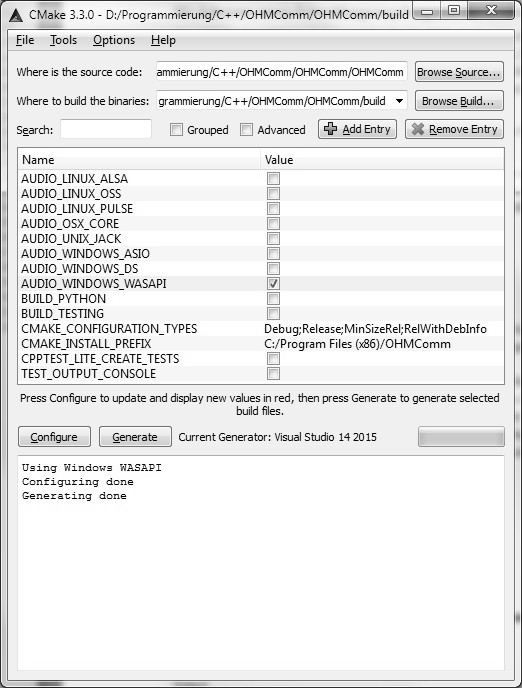
\includegraphics[width=.80\textwidth]{images/CMake}
\caption{CMake Konfiguration unter Windows 7}
\label{Fig:CMake}
\end{figure}

Es wird CMake mitgeteilt wo sich der Source Code \texttt{Browse Source} und das Build Verzeichnis \texttt{Browse Build} befindet \textcolor{red}{SATZ IST FEHLERHAFT}.
Mittels \texttt{Configure} wird der Compiler und die verwendete Entwicklungsumgebung definiert.
Anschließend wird ausgewählt welche Audio Bibliothek verwendet wird, unter Windows wird \textit{ASIO}, \textit{DS} und \textit{WASAPI} unterstützt. Wahlweise kann auch \textit{CppTest} aktiviert werden falls Tests durchführen werden sollen.
Die Einstellungen werden durch nochmaligen Druck auf \texttt{Configure} bestätigt und über \texttt{Generate} werden die Projektdateien im vorher definierten Buildverzeichnis erstellt.

Es wird die \textit{Entwicklungsumgebung} mit den generierten Projekt Dateien gestartet und angewiesen das Projekt zu kompilieren.

Im Verzeichnis \texttt{build/Release/} findet sich bei der Verwendung von Visual Studio und Kompilierung mit Release Optionen das ausführbare Programm \textbf{OHMComm.exe} und die OHMComm Bibliothek \textbf{OHMComm.lib}.

\section{Softwarearchitektur}
\subsection{Konfiguration und Verwendung}
\label{configurationUsages}
Um OHMComm verwenden zu können, müssen vorher eine Vielzahl an Einstellungen getroffen werden. Diese Einstellungen gliedern sich in folgende Bereiche:
\begin{description}
\item[Audio-Konfiguration:]Einstellungen für die Soundkarte, wie die Wahl des Formats zum Aufnehmen oder Abspielen, die Anzahl der Kanäle, die Abtastrate oder die verwendeten Audiogeräte. Die Auswahl der Geräte für die Aufnahme und Ausgabe können unabhängig vom Kommunikationspartner eingestellt werden, die anderen Einstellungen (Audioformat, Kanäle und Abtastrate) müssen jedoch mit dem Gesprächspartner abgestimmt oder auf kompatible Werte umgerechnet werden.
\item[Prozessoren-Konfiguration:]Hierunter fällt die Auswahl der verwendeten Audioprozessoren und die Reihenfolge, in der die Prozessoren verkettet werden (siehe Abschnitt \ref{processingChain}). Ebenso besitzen manche Prozessoren eigene Einstellungsmöglichkeiten, um deren Funktionsweise zu regeln. Die meisten Prozessoren und -Einstellungen fordern keine Anpassung der Konfiguration des Gesprächspartners. Ausnahmen sind hier die Audiocodecs, die von beiden Programmen gleich konfiguriert verwendet werden müssen, um die encodierten Daten wieder richtig decodieren zu können.
\item[Netzwerk-Konfiguration:]Bestimmt den zu verwendeten Port zum Empfangen und Senden von Paketen auf dem lokalen Rechner, sowie die IP-Adresse und den Port des Rechners des Kommunikationspartners. Die Ports und die Adresse des jeweils anderen Rechners müssen vorher zwischen den Gesprächspartner abgestimmt werden, um eine Duplex-Kommunikation einrichten zu können. Bei der Netzwerk-Konfiguration ist zu beachten, dass bei Kommunikation über ein WAN (Wide Area Network) eine von außen erreichbare IP-Adresse gewählt wird evtl. auch Port-Weiterleitungen eingerichtet werden müssen.
\item[Sonstige Konfiguration:] Hier zählen sonstige, rein optionale Einstellungen, die die eigentliche Audiokommunikation nicht beeinflussen, wie das Messen der Ausführungsdauer der verwendeten Prozessoren, das Schreiben des Logs in eine Datei sowie die informativen Daten, die bei RTCP SDES-Paketen gesendet werden (siehe Abschnitt \ref{rtcp}). Da diese Einstellungen nur das lokale Programm betreffen, müssen sie nicht mit dem Gegenüber abgestimmt werden.
\end{description}
Für die meisten nicht-optionalen Einstellungen sind Standardwerte vorgegeben (wie den beiden Ports für den lokalen und entfernten Rechner) oder werden beim Start des Programms ermitteln (wie die Standard-Audiogeräte für die Ein- und Ausgabe). Um die einfachste Form der Kommunikation aufbauen zu können -- ohne Audiocodecs oder sonstigen Audioprozessoren -- muss nur die IP-Adresse des Gegenübers gesetzt werden. jedoch empfiehlt es sich aus verschiedenen Gründen (wie die Reduzierung der Bandbreite) eine erweiterte Konfiguration vorzunehmen.
\\%TODO: nach Steuerung?
OHMComm implementiert eine Vielzahl an Konfigurationsmöglichkeiten, um einen möglichst breiten Verwendungsbereich zu bieten. So kann die prototypische Anwendung aus Kapitel \ref{prototypProgram} als interaktive Konsolen-Anwendung gestartet werden. Dabei werden alle Einstellungsmöglichkeiten nacheinander ausgegeben und der Benutzer kann durch Eingabe einen der vorgeschlagenen Werte auswählen oder einen eigenen Wert eingeben, je nach Art der Einstellung.
\\
Ebenso kann die Konfiguration durch Kommandozeilen-Argumente vorgenommen werden. Hierfür benutzt OHMComm den aus Unix bekannten Syntax, bei dem Schlüssel-Werte Paare mit einem Gleichheitszeichen = getrennt angegeben werden, z.B. \texttt{--local-port=54321} für die Bestimmung des lokalen Ports. Ebenso werden für die meisten Optionen sowohl ein kurzer als auch ein langer Schlüssel unterstützt. So geben beide Argumente \texttt{-h} und \texttt{--help} die Hilfe auf der Kommandozeile aus, die alle verfügbaren Parameter und deren Bedeutung sowie Standard-Werte anzeigt. Die gleichen Parameter können auch aus einer Konfigurationsdatei geladen werden. Dafür werden dort die Schlüssel-Wert Paare zeilenweise und auch durch ein Gleichheitszeichen getrennt (aber ohne führende Bindestriche) aufgelistet und die Datei beim Start an das OHMComm-Programm als einzigen Parameter übergeben.
\\
Um das Programm auch als Bibliothek verwenden zu können, wird eine Möglichkeit geboten, über Methodenaufrufe die benötigten und optionalen Einstellungen zu setzen. %TODO: Verwendung als Bib, Was kanns? Nutzen
\\
Des Weiteren gibt es die sog. \textbf{passive Konfiguration}, bei der alle Konfigurationen, die in beiden Programmen gleich eingestellt sein müssen, vor dem Start der Kommunikation ausgetauscht werden. Zu den ausgetauschten Einstellungen zählen Abtastrate, Audioformat, Anzahl der Kanäle und die verwendeten Prozessoren (für die Audiocodecs). Somit wird die Gleichheit dieser Einstellungen garantiert und der Konfigurationsaufwand verringert. Mehr zur passiven Konfiguration in Abschnitt \ref{rtcp}.
%TODO: Ausführlicher!?

\subsection{Audio-Schnittstelle}
Für die Audioverarbeitung ist ein allgemeine Schnittstelle zur Audiohardware nötig, siehe Anforderung \ref{FA:SchnittstelleAudiohardware}. Dabei gilt es insbesondere die nicht-funktionalen Anforderungen \ref{NFA:Plattformunabhängigkeit}, \ref{NFA:Performanz} und \ref{NFA:Softwarearchitektur} zu berücksichtigen. Es wird eine abstrakte Klasse mit dem Namen \texttt{AudioHandler} erstellt, welche die Verbindung zur Hardware darstellt. Sämtliche Audiodaten laufen über diese Schnittstelle zum Mikrofon oder zu den Lautsprechern. 

\subsubsection{Verarbeitungsmethoden}
Die Klasse bietet drei virtuelle Methoden, welche eine automatische Verarbeitung starten. Die Methode \texttt{start"-Recording"-Mode()} startet die Verarbeitung von Audioinputdaten (Mikrofon), \texttt{start"-Playback"-Mode()} startet die Verarbeitung von Audiooutputdaten (Lautsprecher) und \texttt{start"-Duplex"-Mode()} ist die gleichzeitige Verarbeitung von Audioinput- und Audioutputdaten. Letztere stellt den Standardfall für die Audiokommunikation dar. Wie diese Methoden im Detail aussehen, wird in Unterklassen von \texttt{AudioHandler} implementiert. Für die Hardwareansteuerung ist sinnvoll bereits existierde Lösungen zu verwenden. In diesem Fall kann man Unterklassen von \texttt{AudioHandler} auch als Wrapper-Klasse ansehen.

\subsubsection{Konfiguration}
Vor der Verarbeitung muss die Hardware konfiguriert werden. Hierfür muss das Struct \texttt{AudioConfiguration} verwendet werden. In diesem lassen sich das Mikrofon und die Lautsprecher bestimmen, die Anzahl der Kanäle (Mono - Stereo), die Sample Rate und die Größe des internes Buffers. Der interne Buffer kann vorerst vernachlässigt werden. Im Kapitel von \ref{sec:RTAudio} wird dieser näher erläutert. Für die Übergabe der Einstellungen steht in der Klasse \texttt{AudioHandler} die Methode \texttt{setConfiguration()} zur Verfügung. Falls keine Konfiguration übergeben wird, so wird automatisch die virtuelle Methode \texttt{setDefaultAudioConfig()} aufgerufen. Diese muss ebenfalls von der Unterklasse implementiert werden. Ihre Aufgabe ist es eine Standardkonfiguration zur Verfügung zu stellen, falls die Klasse nicht konfiguriert wurde. Es ist jedoch zu beachten, dass Standardkonfiguration eventuell fehlerhaft und nicht auf allen Systemen lauffähig ist.

\subsubsection{Steuerung der Verarbeitung}
Falls die Verarbeitung läuft kann diese durch Methoden gesteuert werden. Die Methode \texttt{suspend()} pausiert die aktuelle Verarbeitung und \texttt{resume()} setzt sie weiter fort. Die Methode \texttt{stop()} bricht den gesamten Verarbeitungsvorgang ab, welcher anschließend auch nicht mehr mit \texttt{resume()} fortgesetzt werden kann. \texttt{reset()} ruft intern \texttt{stop()} auf und setzt die übergebene Audiokonfiguration zurück.

\subsubsection{Prepare-Methode}
Die virtuelle Methode \texttt{prepare()} nimmt eine Sonderrolle ein. Grundsätzlich kann Sie als optional betrachtet werden, jedoch ist sie für bestimmte Einsatzzwecke sinnvoll. Sie sollte aufgerufen nachdem eine Audiokonfiguration übergeben wurde und bevor die Verarbeitung gestartet ist. Dies kann sinnvoll sein um z.B. die ausgewählte Hardware im Hinblick auf bestimmte Einstellungsmöglichkeiten und deren Kompatiblität mit anderen Komponenten zu überprüfen. Falls eine Inkompatiblität festgestellt wird, kann der Start der Verarbeitung abgebrochen werden.

\FloatBarrier
\subsubsection{Fazit}
Abbildung \ref{Fig:AudioHandlerAnySimple} zeigt eine vereinfachte Darstellung des \texttt{AudioHandlers}. Durch die abstrakte Klasse wird gewährleistet, dass die Klasse austauschbar und erweiterbar ist. Viele Implementierungsdetails werden in die Unterklasse ausgelagert. Durch das Verwenden externer Libraries kann die Unterklasse auch als Wrapper-Klasse angesehen werden. Die Audiohardware lässt sich durch das Struct \texttt{Audio"-Configuration} konfigurieren. Jedoch besteht diese Klasse nicht nur aus der Schnittstelle zur Hardware, sondern ist der zentraler Verarbeitungspunkt, daher einer der wichtigsten Komponenten des Frameworks. Für die Verarbeitung von Audiodaten wurde eine spezielle Schnittstelle, die Verarbeitungskette, integriert. Im folgenden Kapitel wird diese näher erläutert.
\newline
\begin{figure}[htp]
\centering
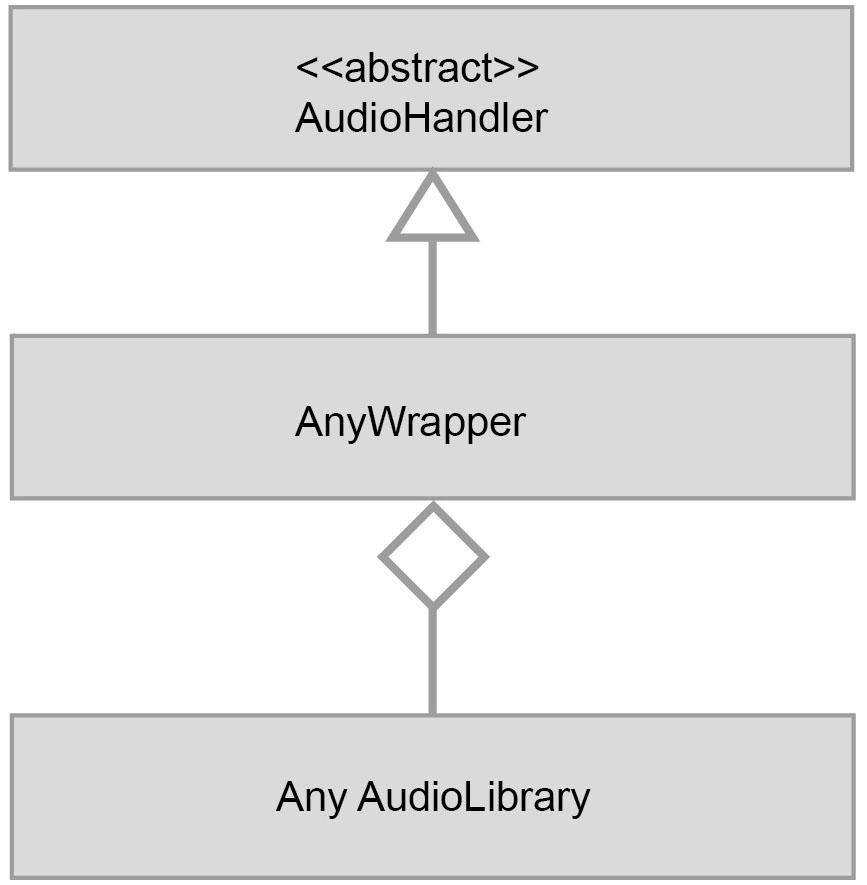
\includegraphics[width=.45\textwidth]{../img/AudioHandlerAnySimple}
\caption{UML-Klassendiagramm des AudioHandlers}
\label{Fig:AudioHandlerAnySimple}
\end{figure}

\FloatBarrier
\subsection{Verarbeitungskette}
\label{processingChain}

Die Klasse \texttt{AudioHandler} bietet eine Schnittstelle zur Hardware an. Ein Teil ihrer Implementierung ist die Verarbeitungskette. Durch ihr können andere Klassen mit den Audiodaten arbeiten, ohne die Implementierungsdetails des \texttt{AudioHandlers} kennen zu müssen. Im folgenden Abschnitt wird erklärt wie diese funktioniert.

\FloatBarrier
\subsubsection{AudioProcessor}
Wenn eine Klasse mit den Audiodaten arbeiten will, so muss sie das Interface \texttt{AudioProcessor} implementieren, siehe Abbildung \ref{Fig:AudioProcessorExample}. Hierfür muss sie die Methoden \texttt{process"-Input"-Data()} und \texttt{process"-Output"-Data()} implementieren. \texttt{process"-Input"-Data()} wird immer aufgerufen, wenn Audiodaten vom Mikrofon für die Verarbeitung im internen Buffer vorhanden sind. Wenn der zweite interne Buffer zum Abspielen von Audiodaten leer ist, wird die Methode \texttt{process"-Output"-Data()} aufgerufen. Dort können Daten auf den Buffer zum Abspielen hinterlegt werden. Beide Funktionen haben als Parameter den jeweiligen Buffer und die Größe des Buffers. Der Rückgabewert der Funktion ist die neue oder alte Größe des Buffers. Der Rückgabewert ist nur auf Hinblick des Dekodieren und Kodieren relevant.
\newline
\begin{figure}[htp]
\centering
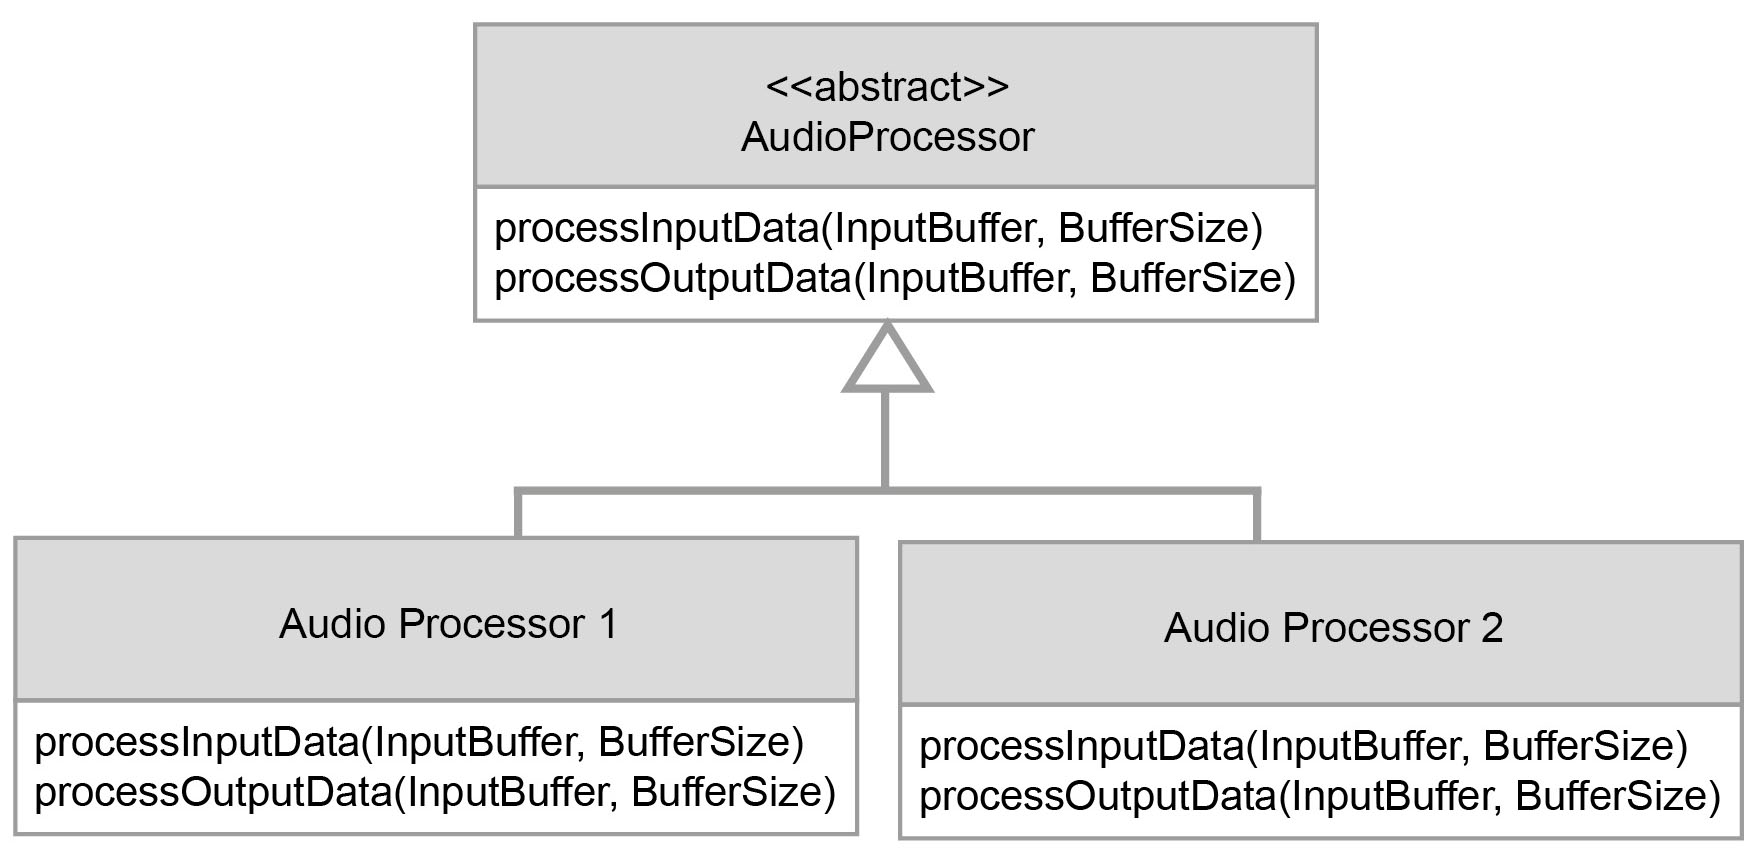
\includegraphics[width=1\textwidth]{../img/AudioProcessorExample}
\caption{Beispielhafte Verwendung der AudioProcessor-Klasse}
\label{Fig:AudioProcessorExample}
\end{figure}

\texttt{configure()} und \texttt{cleanUp()} sind weitere Methoden des AudioProcessors, die nicht in der Abbildung \ref{Fig:AudioProcessorExample} zu sehen sind. Erstere wird einmalig, kurz bevor die Verarbeitung startet, aufgerufen. Als Parameter muss die festgelegte Audiokonfiguration übergeben werden. Die Funktion hat einen boolschen Rückgabewert der angibt, ob der AudioProcessor bereit für die Audioverarbeitung ist. Im Fehlerfall startet die Verarbeitung nicht. Dies kann wichtig sein, wenn z.B. ein \texttt{AudioProcessor} eine gewisse Audiokonfiguration voraussetzt. \texttt{cleanUp()} dient dazu, den \texttt{AudioProcessor} ordentlich aufzuräumen, wenn dieser nicht mehr benötigt wird.

\FloatBarrier
\subsubsection{Registrieren von Audioprozessoren}
Das Implementieren der Klasse \texttt{AudioProcessor} reicht nicht aus, um an der Audioverarbeitung aktiv teilzunehmen. Abbildung \ref{Fig:AudioHandlerAudioProcessor} zeigt die Beziehung zwischen \texttt{Audio"-Handler} und \texttt{Audio"-Processor}. Die Klasse muss sich beim \texttt{AudioHandler} mit der Methode \texttt{addProcessor()} anmelden. Diese nimmt als Parameter einen \texttt{AudioProcessor} entgegen. Audioprozessoren lassen sich über ihren Namen eindeutig identifizieren. Der Prozessor wird, falls er schon nicht vorhanden ist, in einer Liste vom Typ \texttt{AudioProcessor} eingefügt. Falls nun Audioinputdaten anliegen, so werden von allen Audioprozessoren, die sich in der Liste befinden, die \texttt{process"-Input"-Data()}-Methoden aufgerufen. Die Aufrufreihenfolge ist abhängig von der Anmeldereihenfolge. Für Audiooutput-Daten geschieht das analog, jedoch ist hier die Aufrufreihenfolge entgegengesetzt, da die Verarbeitungskette nicht kommutativ ist. Nur so ist es möglich an die ursprünglichen Audiodaten zu gelangen. Das Konzept hat einige Vorteile, wie z.B. beliebige viele Prozessoren können sich beim \texttt{AudioHandler} anmelden, jedoch hierbei der Aspekt der Performanz zu berücksichtigen. Des weiteren können Audioprozessoren zur Laufzeit hinzugefügt werden und beeinflussen sich nicht gegenseitig. Änderungen am \texttt{AudioHandler} sind ebenfalls unabhängig von den Prozessoren.
Vom Aufbau ähnelt die Verarbeitungskette dem Observer-Pattern, jedoch mit dem entscheidenden Unterschied, dass die Einfügereihenfolge eine wesentliche Rolle für die Verarbeitung spielt. 
\newline
\begin{figure}[htp]
\centering
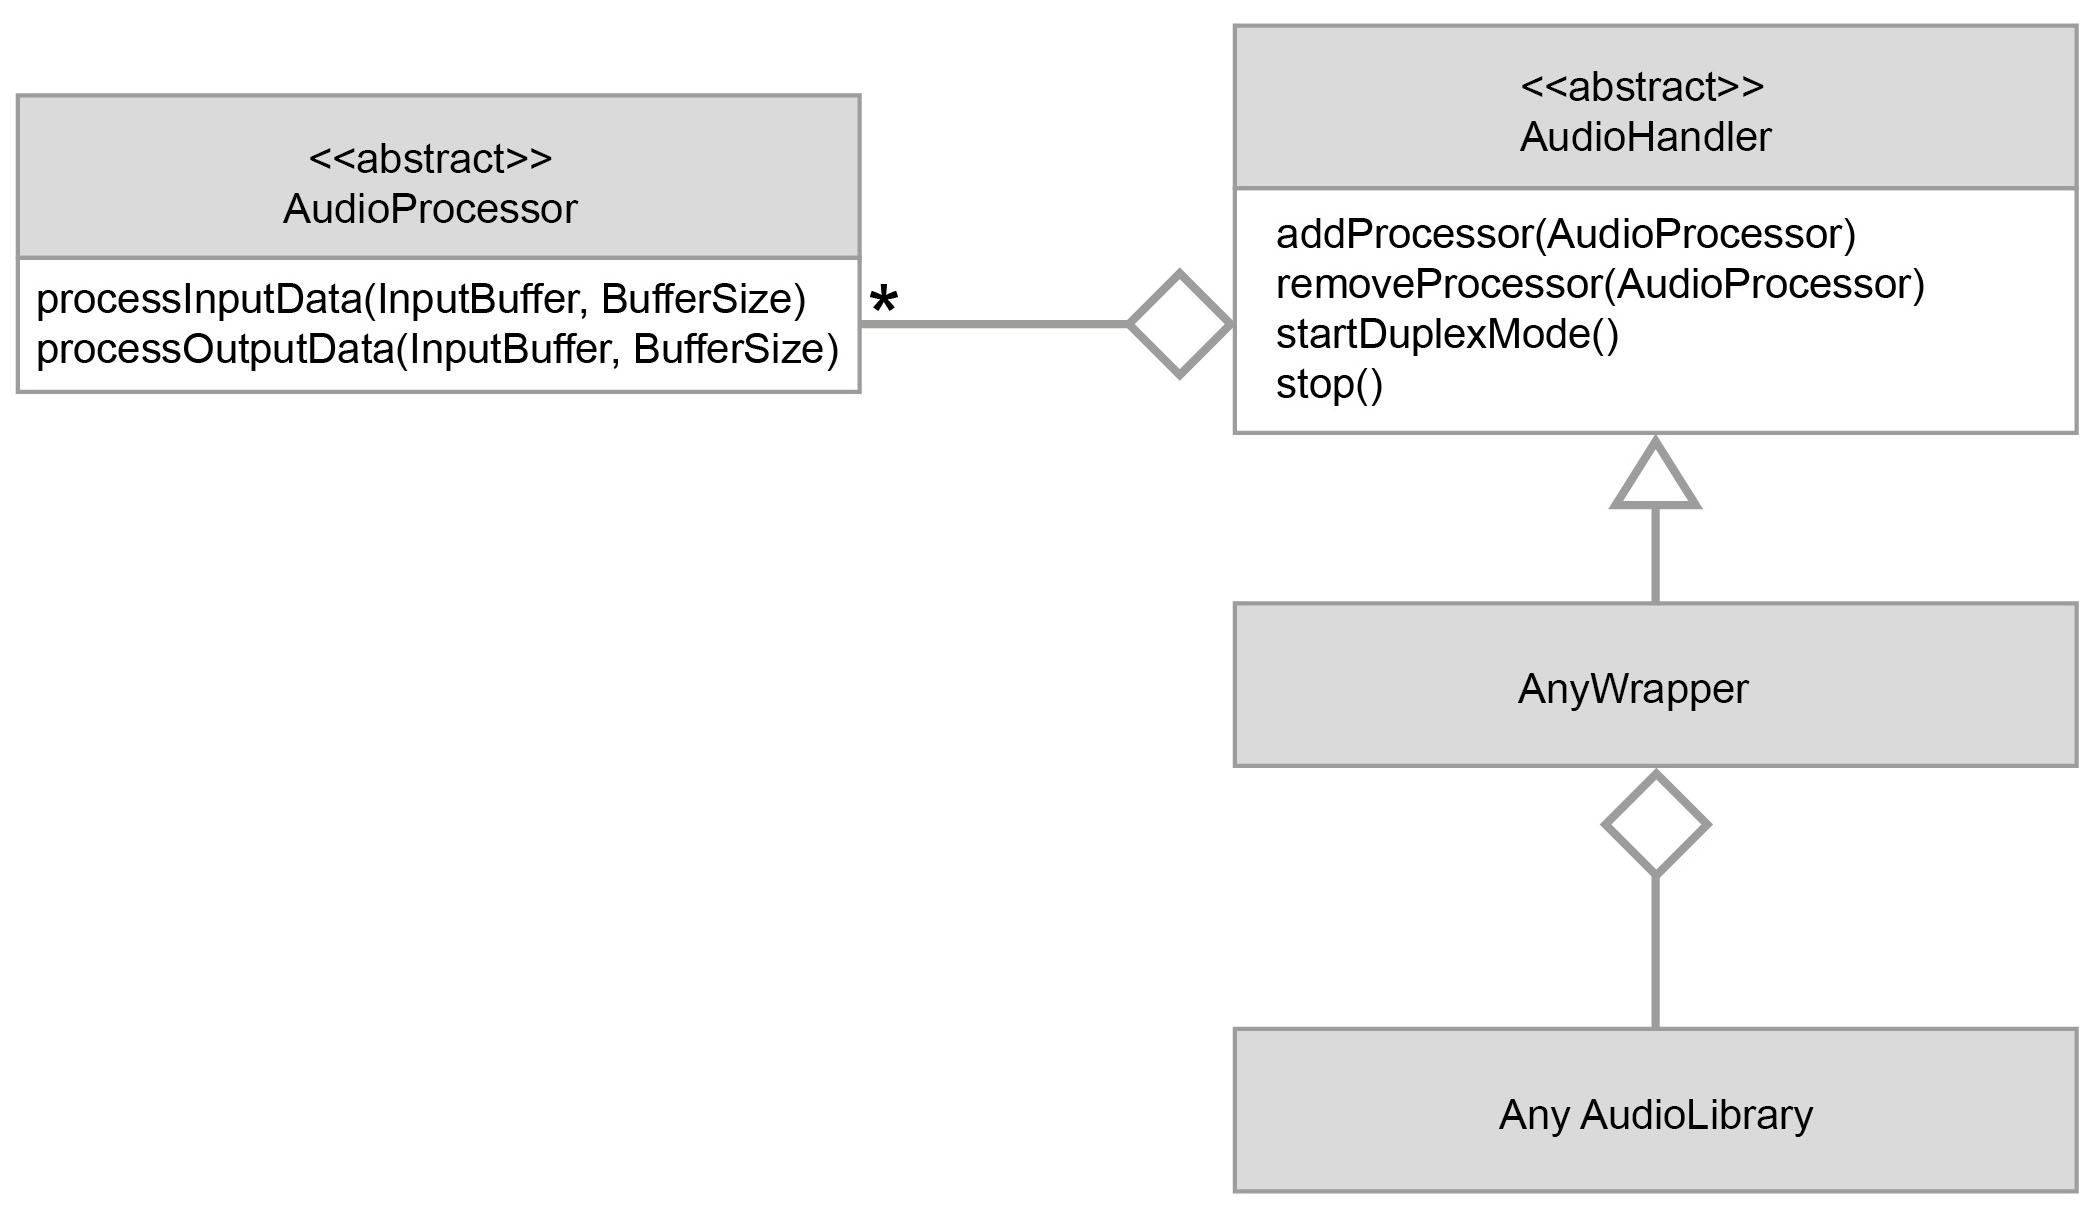
\includegraphics[width=1\textwidth]{../img/AudioHandlerAudioProcessor}
\caption{UML-Klassendiagramm AudioHandler und AudioProcessors}
\label{Fig:AudioHandlerAudioProcessor}
\end{figure}

\FloatBarrier




\subsubsection{ProfilingAudioProcessor}
Beim \texttt{Profiling"-AudioProcessor} handelt es sich um eine spezielle Unterklasse des \texttt{AudioProcessors}, siehe Abbildung \ref{Fig:ProfilingAudioProcessor}. Der Prozessor hat die Aufgabe Anforderung \ref{FA:Statistik} umzusetzen. Die Umsetzung erfolgt mit dem Decorator-Pattern. Dieses ermöglicht es ein Objekt dynamisch zur Laufzeit zu erweitern. Der \texttt{Profiling"-AudioProcessor} ist dabei zum einem Unterklasse des zu erweiterten Objekt und zum anderen hat es eine Referenz darauf. Der Konstruktor des \texttt{Profiling"-AudioProcessor} nimmt als Parameter einen Pointer vom Typ \texttt{AudioProcessors} entgegen und speichert die Referenz. Der \texttt{Profiling"-AudioProcessor} muss die Methoden der Oberklasse implementieren, jedoch werden deren Aufrufe an die gespeicherte Referenz des \texttt{AudioProcessors} weitergeleitet. Funktionen die erweitert werden sollen, können vor und nach der Delegation ergänzt werden.
\newline
\begin{figure}[htp]
\centering
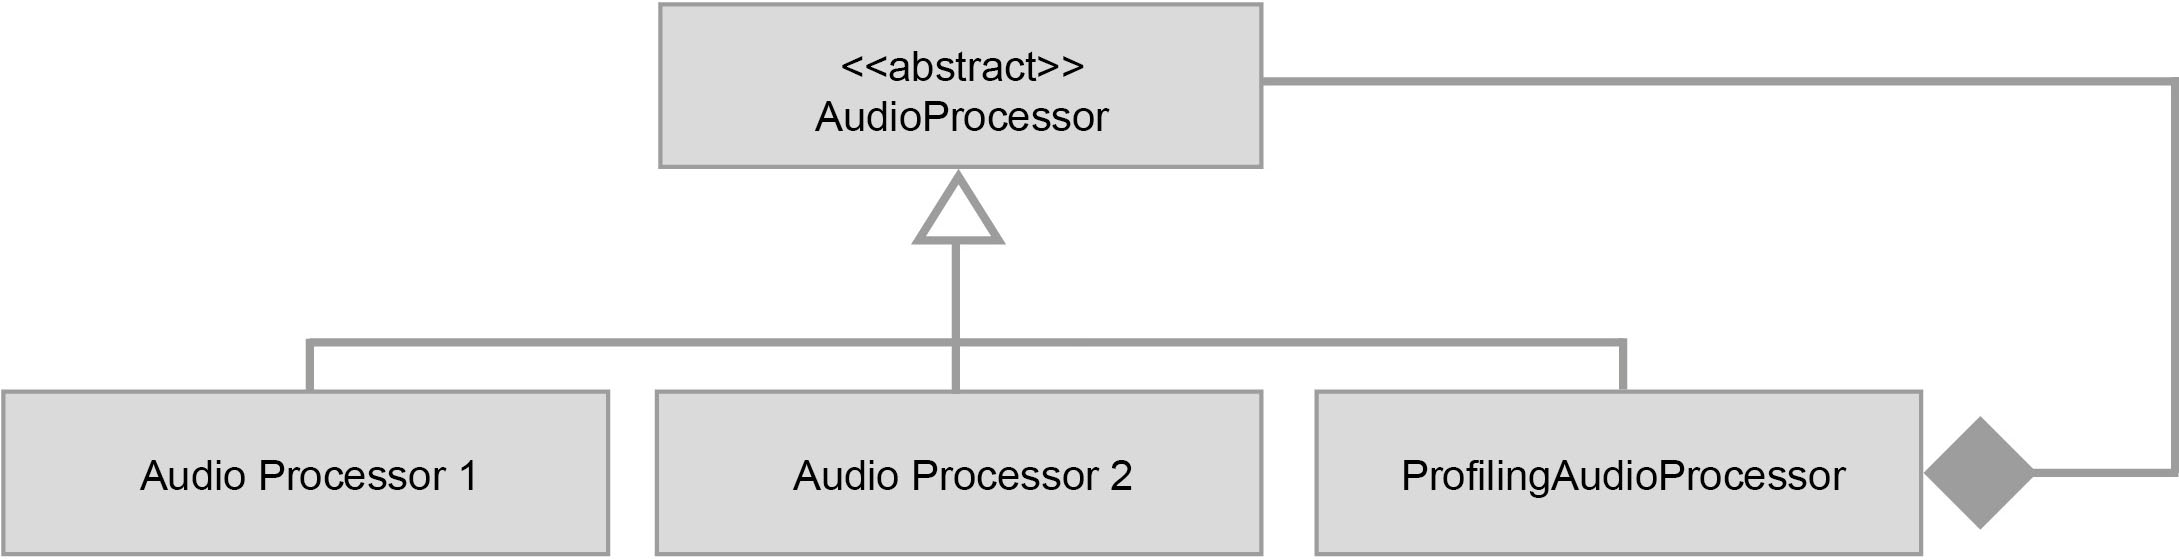
\includegraphics[width=1\textwidth]{../img/ProfilingAudioProcessor}
\caption{UML-Klassendiagramm des ProfilingAudioProcessors}
\label{Fig:ProfilingAudioProcessor}
\end{figure}

\FloatBarrier

\subsection{Austauschbarkeit und Instantiierung}
Um der Anforderung \ref{NFA:Softwarearchitektur} gerecht zu werden und die Komponenten austauschbar zu halten, wird das Entwurfsprinzip \texttt{Program to an interface, not to an implementation} \cite{Lahres2009}[Kap. 3.5] umgesetzt. Dies ermöglicht eine höhere Flexibilität, da der abstrakte Typ zur Laufzeit durch ein konkretes Objekt ausgetauscht werden kann. In diesem Zusammenhang bietet es sich an das Factory-Method-Pattern zu integrieren. Dabei wird die Instantiierung in einer Fabrikmethode ausgelagert. Als Parameter erwartet die Funktion ein String mit dem Namen der zu instantiierten Klasse. Alle Klassen basieren auf den gemeinsamen abstrakten Basistypen, der auch gleichzeitig Rückgabetyp ist. Die Fabrikmethoden wurde in eigenen Fabrikklassen ausgelagert, wie in Abbildung \ref{Fig:Factories} zu sehen ist. \texttt{getAudioHandler()} und \texttt{getAudioProcessor()} stellen die Fabrikmethoden dar. \texttt{getAudioHandlerNames()} und \texttt{getAudioProcessorNames()} liefern die Namen der Klassen, die instantiierbar sind.
\newline
\begin{figure}[htp]
\centering
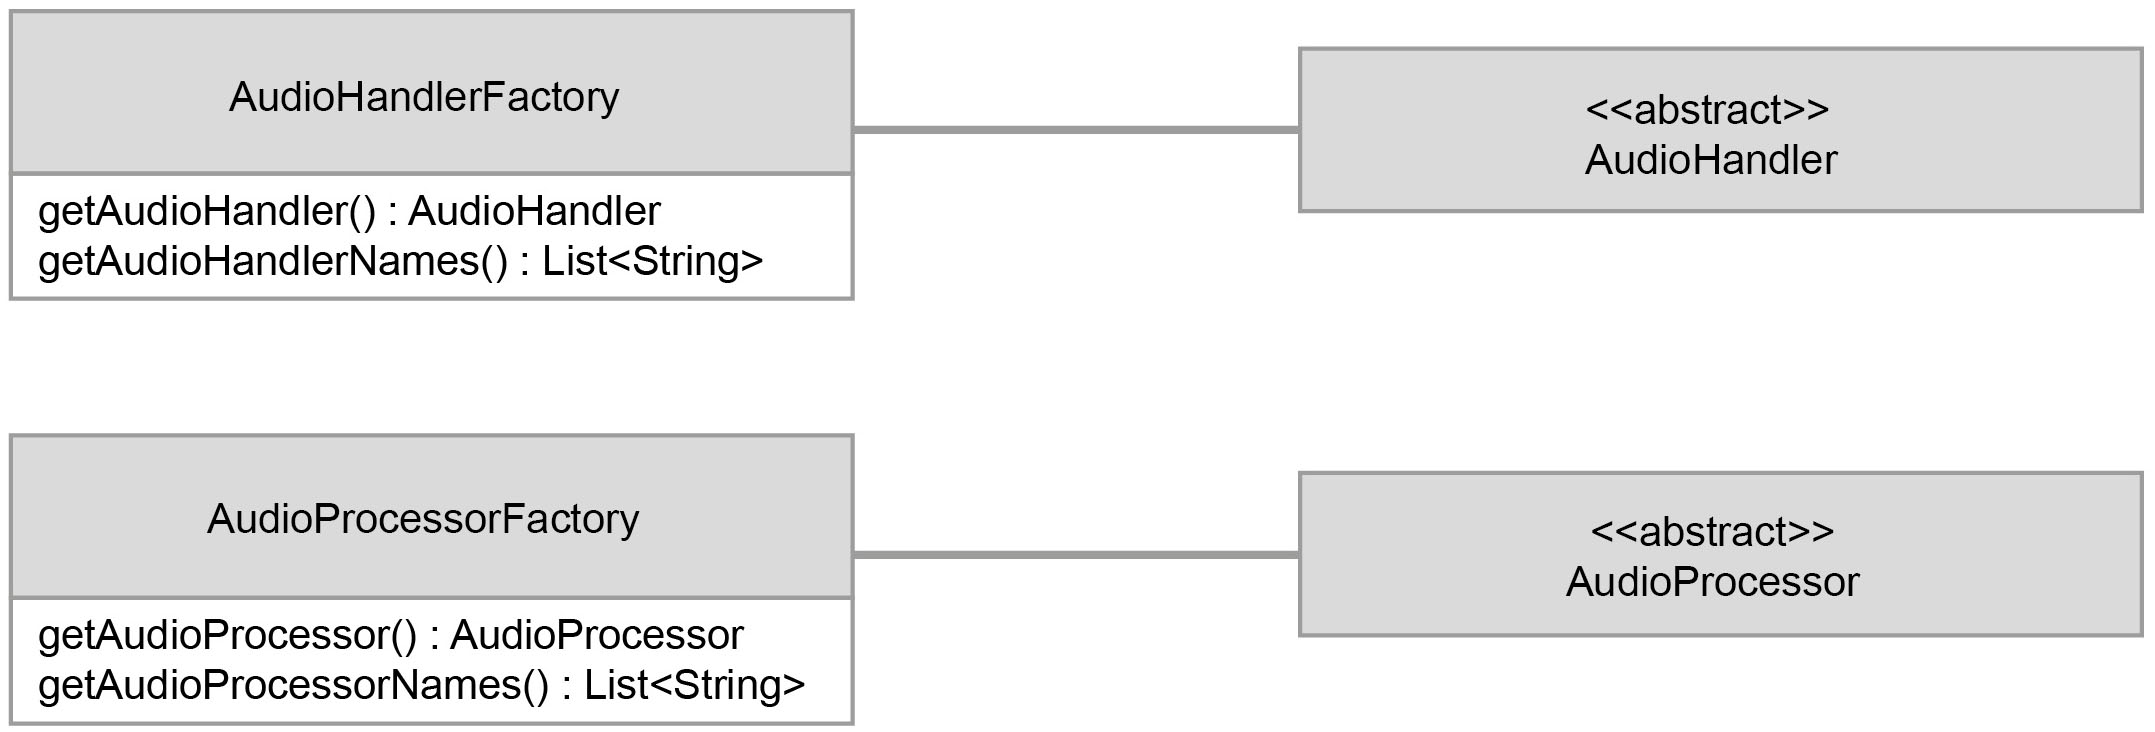
\includegraphics[width=1\textwidth]{../img/Factories}
\caption{Factory-Klassen im Überblick}
\label{Fig:Factories}
\end{figure}

\FloatBarrier

\subsection{RTP-Protokoll}
\label{rtp}
Das Real-time Transport Protocol (RTP) ist ein Netzwerkprotokoll für die Übertragung von Echtzeitdaten, wie Audio- und Videostreams oder -Konversationen, ist im RFC 3550 der Internet Engineering Task Force (IETF) definiert (siehe \cite{RFC3550}) und unterstützt sowohl Unicast- als auch Multicast-Sitzungen. RTP ist ein Protokoll für die Anwendungsebene und kann auf beliebigen Transportprotokollen wie UDP oder TCP aufgesetzt werden. Jedoch wird RTP meist mit UDP verwendet, da aufgrund der Echtzeitvoraussetzungen der Verlust von Paketen erträglicher ist als das Blockieren weiterer Daten durch erneutes Senden nicht-angekommener Pakete, so wie es in TCP üblich ist. Dies hat wiederum zur Folge, dass eine auf RTP mit UDP basierende Anwendung den Verlust einzelner Pakete kompensieren muss. Ein RTP-Paket besteht aus dem RTP-Header und dem anwendungsspezifischen Payload (Body). Der RTP-Header hat eine Größe von zwölf bis 72 Bytes und definiert folgende Felder:
\begin{lstlisting}[keepspaces=true,numbers=none,label=lst=rtpHeader,caption=RTP Header \cite{RFC3550}]
 0                   1                   2                   3
 0 1 2 3 4 5 6 7 8 9 0 1 2 3 4 5 6 7 8 9 0 1 2 3 4 5 6 7 8 9 0 1
+-+-+-+-+-+-+-+-+-+-+-+-+-+-+-+-+-+-+-+-+-+-+-+-+-+-+-+-+-+-+-+-+
|V=2|P|X|  CC   |M|     PT      |       sequence number         |
+-+-+-+-+-+-+-+-+-+-+-+-+-+-+-+-+-+-+-+-+-+-+-+-+-+-+-+-+-+-+-+-+
|                           timestamp                           |
+-+-+-+-+-+-+-+-+-+-+-+-+-+-+-+-+-+-+-+-+-+-+-+-+-+-+-+-+-+-+-+-+
|           synchronization source (SSRC) identifier            |
+=+=+=+=+=+=+=+=+=+=+=+=+=+=+=+=+=+=+=+=+=+=+=+=+=+=+=+=+=+=+=+=+
|            contributing source (CSRC) identifiers             |
|                             ....                              |
+-+-+-+-+-+-+-+-+-+-+-+-+-+-+-+-+-+-+-+-+-+-+-+-+-+-+-+-+-+-+-+-+
\end{lstlisting}
\begin{description}
\item[Version:] Hat in RFC 3550 immer den Wert 2, frühere Versionen hatten den Wert 1.
\item[Padding-Bit:] Gibt an, ob die Daten des RTP-Pakets auf ein Vielfaches von 4 Byte gepadded sind.
\item[Extension-Bit:] Gibt an, ob eine RTP Header-Extension existiert, die direkt an den Header anschließt.
\item[CSRC Count:] Gibt die Anzahl der Contribution Sources (CSRCs) an, maximal 15 aufgrund der Größe des Feldes mit 4 Bit.
\item[Marker-Bit:] Anwendungsspezifische Bedeutung.
\item[Payloadtype:] Gibt den Typ der transportierten Daten an. Dieser kann aus einer Liste vordefinierter Typen aus RFC 3551 oder dynamisch ausgewählt sein.
\item[Sequence number:] Gibt die Position des RTP-Pakets innerhalb des Datenstroms an und wird für die Umsortierung der Pakete verwendet. Der Anfangswert dieses Felds sollte zufällig gewählt werden.
\item[Timestamp:] Zeitpunkt, zu dem das erste Byte des Pakets erstellt wurde, wobei auch hier der Anfangswert zufällig gewählt wird.
\item[Synchronization Source Identifier:] Zufällig gewählte Zahl zum eindeutigen identifizieren des Senders dieses Pakets, auch SSRC genannt.
\item[Contribution Source Identifier:] Beinhaltet die originalen SSRCs der Teilpakete, wenn das Paket von einem Mixer aus verschiedenen Teilpaketen zusammengestellt wurde, werden auch CSRCs abgekürzt.
\end{description}
Im OHMComm-Framework wird RTP auf Basis von UDP verwendet, um den Verlust von Paketen zu Entdecken und eine Sortierreihenfolge festzulegen. Da OHMComm keine Sitzungen mit mehr als zwei Teilnehmern oder verschiedene Payload-Typen innerhalb einer Sitzung unterstützt, haben die meisten Header-Felder für das Framework keine Bedeutung. Jedoch werden für gesendete RTP-Pakete alle Header-Felder richtig belegt, um eine Interoperabilität mit anderen VoIP-Programmen zu gewährleisten. Für das Auslesen und Erstellen von RTP-Paketen sowie generieren der richtigen Header-Felder ist die Klasse \texttt{RTPPackageHandler} verantwortlich. So könnte man z.B. mithilfe von OHMComm eine  Sitzung mit mehreren Teilnehmern aufbauen, indem der lokale Client mit einem RTP-Mixer kommuniziert, der die Pakete dann auf die anderen Teilnehmer verteilt und auch deren Pakete vereint.
\subsubsection{RTCP-Protokoll}
\label{rtcp}
Das Real-time Transport Control Protocol (RTCP) ist auch in RFC 3550 definiert und bietet Möglichkeiten Flusskontrolle für eine RTP-Sitzung durchzuführen sowie statistische Daten über die Verbindungsqualität (oder Quality of Service, kurz: QoS) zu übertragen. Ebenso werden Pakettypen für anwendungsspezifische Daten und zum Beenden einer RTP-Sitzung bereitgestellt. Im Gegensatz zu RTP-Paketen beinhalten RTCP-Pakete keine Daten, sondern bestehen nur aus RTCP-Headern. Jedoch ist in RFC 3550 vorgegeben, dass ein RTCP-Header nie einzeln, sondern nur in Gruppen von mindestens zwei Headern, sogenannten \enquote{compound packages}, versendet wird. Die verschiedenen RTCP-Pakettypen bestehen aus den ersten acht Bytes, die für alle Typen die gleiche Bedeutung haben, sowie einen Typ-spezifischen Teil. Der gemeinsame Header-Teil besteht aus den folgenden Feldern:
\begin{lstlisting}[keepspaces=true,numbers=none,label=lst=rtcpHeader,caption=RTCP Header \cite{RFC3550}]
 0                   1                   2                   3
 0 1 2 3 4 5 6 7 8 9 0 1 2 3 4 5 6 7 8 9 0 1 2 3 4 5 6 7 8 9 0 1
+-+-+-+-+-+-+-+-+-+-+-+-+-+-+-+-+-+-+-+-+-+-+-+-+-+-+-+-+-+-+-+-+
|V=2|P|    RC   |      PT       |             length            |
+-+-+-+-+-+-+-+-+-+-+-+-+-+-+-+-+-+-+-+-+-+-+-+-+-+-+-+-+-+-+-+-+
|                     SSRC of packet sender                     |
+=+=+=+=+=+=+=+=+=+=+=+=+=+=+=+=+=+=+=+=+=+=+=+=+=+=+=+=+=+=+=+=+
\end{lstlisting}
\begin{description}
\item[Version:] Hat in RFC 3550 immer den Wert 2, frühere Versionen hatten den Wert 1.
\item[Padding-Bit:] Gibt an, ob der RTCP-Header auf ein Vielfaches von 4 Byte gepadded ist. Padding darf nur das letzte Teilpaket eines zusammengesetzten Pakets angewendet werden.
\item[Item Count:] Gibt die Anzahl der Einträge in diesem RTCP-Header an. Die Bedeutung hiervon ist abhängig vom Pakettyp
\item[Package Type:] Gibt den Typ des RTCP-Paketes an
\item[length:] Die Länge des RTCP-Teilheaders in 32-Bit Blöcken, minus 1 (den ersten 32-Bit Block)
\item[SSRC:] Source Description des Senders, stimmt mit der SSRC von RTP-Paketen dieses Senders überein
\end{description}
RFC 3550 definiert folgende RTCP Pakettypen und deren Inhalten:
\begin{description}
\item[Sender Report:] Beinhaltet Informationen über die Anzahl an gesendeten Paketen und Daten eines Senders. Ebenso werden pro Teilnehmer, von dem der Sender des Sender Reports Pakete empfangen hat, Daten über die Quality of Service (Anzahl verlorener Paketen, Netzwerkjitter, letzter empfangener Sender Report) verschickt. Diese Reception Report genannten Blöcke ermöglichen, dass jeder Teilnehmer einer RTP-Sitzung von jedem anderen Teilnehmer in regelmäßigen Abständen Feedback über die Übertragungsqualität bekommt. Jeder aktive Sender in einer RTP-Sitzung muss alle zusammengesetzten RTCP-Pakete immer mit einem Sender Report beginnen.
\item[Receiver Report:] Äquivalent zum Sender Report für passive Teilnehmer (also Teilnehmer die selbst keine Daten verschicken). Beinhaltet keine Informationen zur Anzahl verschickter Daten, aber trotzdem die Liste der Reception Reports für alle anderen Sender. Jeder passive RTP-Teilnehmer muss ein zusammengesetztes Paket immer mit einem Receiver Report beginnen.
\item[Source Description:] Beinhaltet eine Liste an informativer Daten über den Teilnehmer mit der angegebenen SSRC. Diese Daten, wie Telefonnummer, E-Mail, Webseite und Name können von Client-Programmen für die anderen Teilnehmer einer Sitzung angezeigt werden.
\item[BYE:] Der BYE RTCP-Header benachrichtigt die Teilnehmer einer Sitzung, dass der Sender mit der angegebenen SSRC die Sitzung verlässt und muss immer als letztes Paket eines zusammengesetzten Pakets stehen.
\item[Application-defined:] Der letzte Pakettyp bietet die Möglichkeit, anwendungsspezifische Daten zu übertragen. Dafür wird ein Name zur Identifikation des Typs der Daten und eine variable großer Block für die eigentlichen Daten bereitgestellt.
\end{description}
Im OHMComm-Framework werden RTCP-Pakete in der Klasse \texttt{RTCPPackageHandler} erstellt sowie ausgelesen und in \texttt{RTCPHandler} verschickt und empfangen. \texttt{RTCPHandler} besitzt einen eigenen Thread, der auf einem dedizierten RTCP-Port auf ankommende Pakete wartet sowie in regelmäßigen Abständen (oder wenn explizit dazu aufgefordert) RTCP-Pakete verschickt. Folgende Pakettypen werden von der RTCP-Implementierung verwendet:
\\
In regelmäßigen Abständen wird ein zusammengesetztes Paket aus \textbf{Sender Report} (mit einem Reception Report) und \textbf{Source Description} versendet, wie es RFC 3550 vorschreibt. Jede empfangenen Sender Report oder Source Description Pakete werden in der prototypischen Anwendung derzeit nicht weiter verarbeitet, sondern nur auf der Konsole ausgegeben. Wenn die OHMComm-Anwendung beendet wird, wird zu den beiden genannten Pakettypen ein \textbf{BYE}-Paket angehängt, das auf der Empfänger-Seite dafür sorgt, dass die Kommunikation auch dort ordnungsgemäß abgebaut wird. Somit wird beim Beenden eines der Klienten der andere auch beendet, zumindest für die Kommunikation zwischen zwei OHMComm-Frameworks. Zusätzlich wird für die \textbf{passive Konfiguration} aus Abschnitt \ref{configurationUsages} der \textbf{Application-defined} Pakettyp verwendet, um eine Konfigurationsanfrage zu stellen und die geteilten Einstellungen auszutauschen. TODO: Der genaue Ablauf der passiven Konfiguration wird in Abschnitt (Impl oder prototyp. Anwendung) beschrieben.

\subsection{Jitter-Buffer}
Wie bereits in Abschnitt \ref{rtp} erwähnt, wird eine Echtzeitübertragung mit RTP meist mit dem Transportprotokoll UDP verwendet. Da UDP aber nicht garantiert, dass versendete Pakete beim Empfänger ankommen und auch nicht, in welcher Reihenfolge, muss die Anwendung dafür sorgen, dass mit verlorenen Paketen oder Paketen, die in der falschen Reihenfolge empfangen werden, richtig umgegangen wird. Dafür gibt es auf der Empfängerseite einen Jitter-Buffer, einen Puffer, der empfangene Pakete speichert und aus dem die weitere Prozessorkette Pakete in der richtigen Reihenfolge auslesen kann. Der Begriff Jitter-Buffer kommt von dem englischen Wort Jitter, dass für die Netzwerkverzögerung, oder genauer: die Varianz der Netzwerkverzögerung steht. Wie der Name schon andeutet, ist es eine der Aufgaben eines Jitter-Buffers, die Verzögerung des Netzwerkes und deren Schwankung auszugleichen. Ebenso sortiert ein Jitter-Buffer die empfangenen Pakete anhand ihrer RTP Sequenz-Nummer um und kaschiert den Verlust von Paketen. Bei Bibliotheken oder Programmen, die Sitzungen mit mehreren Teilnehmern unterstützen -- was bei OHMComm nicht der Fall ist -- muss für jeden anderen Sender ein eigener Jitter-Buffer verwaltet werden, da die Pakete der verschiedenen Sender verschiedene Netzwerkverzögerungen aufweisen können.
\\
Bei der Netzwerkübertragung über UDP können Pakete verloren gehen, oder sie werden so spät empfangen, dass sie bereits hätten abgespielt werden müssen, sog. \enquote{late loss}. Um den Audiotreiber trotzdem Daten zum Abspielen zu liefern, und nicht die Ausgabe ins Stocken zu bringen, muss ein Echtzeitkommunikationsprogramm dafür sorgen, dass diese Verluste von Audiodaten ausgeglichen werden. Diese Funktion nennt sich \enquote{loss concealment} (also: Verstecken von Verlusten) und kann auf verschiedene Arten umgesetzt werden. Die einfachste Möglichkeit ist es, wenn ein Paket angefordert wird, dass (noch) nicht empfangen worden ist, die Audiodaten dieses Pakets mit \textbf{Stille} zu ersetzen. Stille lässt sich sehr einfach erzeugen (z.B: durch Setzen aller Samples auf Null), ist ab einer gewissen Dauer für den Menschen hörbar und unterbricht den Fluss des Gesprächs, das Gespräch kling abgehakt. Als weitere Möglichkeit kann anstatt der Stille ein zufällig generiertes leises Rauschen, sog. \enquote{\textbf{comfort noise}}, abgespielt werden. Im Gegensatz zur absoluten Stille bekommt man bei Rauschen nicht so schnell das Gefühl, dass die Verbindung abgebrochen ist. Eine dritte Möglichkeit wiederholt das letzte erfolgreich empfangene Paket und spielt es erneut ab. Da sich der Tonverlauf der menschlichen Stimme nicht so schnell ändert, %TODO ca. Zeitdauer
besteht eine große Wahrscheinlichkeit, dass die Audiodaten des verlorene Pakets dem vorherigen sehr ähnlich sind und der Unterschied kaum hörbar wird. Alle drei dieser einfachen Methoden für \enquote{loss concealment} sind einfach zu implementieren und besitzen eine geringe Laufzeit, werden dafür vor Allem bei längeren Stille-Perioden sehr schnell hörbar und stören den Gesprächsverlauf. Deshalb gibt es noch eine Vielzahl weiterer Algorithmen, die versuchen, Unterbrechungen möglichst unhörbar zu überdecken, dies jedoch meist auf Kosten erhöhter Laufzeit und Komplexität erkaufen.
\\
Um den Verlust von Paketen aufgrund von \enquote{late loss} gering zu halten und somit eine flüssige und möglichst vollständige Audiokommunikation zu gewährleisten, führt ein Jitter-Buffer eine künstliche Verzögerung zwischen dem Empfangen und dem Abspielen eines Paketes ein. Dadurch, dass ein Paket später abgespielt wird (der sog. \enquote{playout point} wird nach Hinten verschoben), hat es länger Zeit, beim Empfänger anzukommen, wodurch weniger Pakete wegen \enquote{late loss}, also dem Ankommen nach ihrem \enquote{playout point}, verworfen werden. Hierfür sollte die Abspielverzögerung so gewählt werden, dass möglichst alle Pakete, die nicht auf dem Netzwerk verloren gehen, den Empfänger vor ihrem Abspielzeitpunkt erreichen. Auf der anderen Seite darf die Abspielverzögerung nicht zu groß werden, sonst leidet die Qualität der Echtzeitkommunikation. Dafür wird in umfangreicheren Implementierungen die Abspielverzögerung meist dynamisch angepasst. Diese sog. \enquote{playout point adaption} wird auf Basis des Anteils an \enquote{late loss} berechnet und in bestimmten Abständen durch einschieben eines zusätzlichen Pakets (z.B. Stille) oder überspringen eines empfangenen Paketes umgesetzt. Der Jitter-Buffer des OHMComm-Frameworks heißt \texttt{RTPBuffer} und besitzt eine feste Abspielverzögerung, die derzeit noch bei der Kompilierung des Programms eingestellt werden muss.
\subsection{Netzwerkverbindung}
Wie auch die meisten anderen Komponenten des OHMComm-Framework (Audio-Bibliothek, -Prozessoren) ist auch die Umsetzung der Netzwerkschnittstelle austauschbar implementiert. Dies wird durch die abstrakte Basisklasse \texttt{NetworkWrapper} umgesetzt, die Methodensignaturen zum Senden und Empfangen von Daten sowie zum Schließen der Verbindung bereitstellt. Bei einer Implementierung einer Netzwerkschnittstelle muss dafür gesorgt werden, dass die Senden- und Empfangen-Methoden keine Data-Races erzeugen können, da diese eventuell aus verschiedenen Threads heraus aufgerufen werden. Da RTP in den allermeisten Fällen mit dem Transportprotokoll UDP verwendet wird, gibt es jedoch derzeit nur eine konkrete Implementierung der Netzwerkschnittstelle namens \texttt{UDPWrapper}, die RTP-Pakete in UDP-Pakete verpackt und beim Empfangen wieder entpackt. Spätere Versionen des Frameworks enthalten zusätzlich noch eine Implementierung, die TCP verwendet.

\FloatBarrier
\subsection{RTPListener}
Die Socketmethoden zum Empfangen von Paketen sind blockierend \cite{WinsockReference}. Dies hat weitreichende Folgen für die Architektur. Der Ausgangspunkt der Verarbeitung ist die Verarbeitungskette im \texttt{Audio"-Handler}. Wird dort eine blockierende Funktion aufgerufen, so wird die gesamte Weiterverarbeitung blockiert. Wenn z.B. innerhalb eines Audioprozessors die blockierende Winsock-Funktion \texttt{recv"-from()} aufgerufen wird, und es werden keine Pakete empfangen, dann bricht die gesamte Verarbeitung ab. Dieses Verhalten ist nicht erwünscht. Die Verarbeitung soll unabhängig von den empfangenen Paketen funktionieren. Die Klasse \texttt{RTPListener} stellt einen Lösungsansatz für dieses Problem dar. Hierfür wird der gesamte Empfangsprozess in einem eignen Thread ausgelagert. Abbildung \ref{Fig:RTPListenerAdvanced} zeigt den Aufbau des \texttt{RTPListeners}.
\newline
\begin{figure}[htp]
\centering
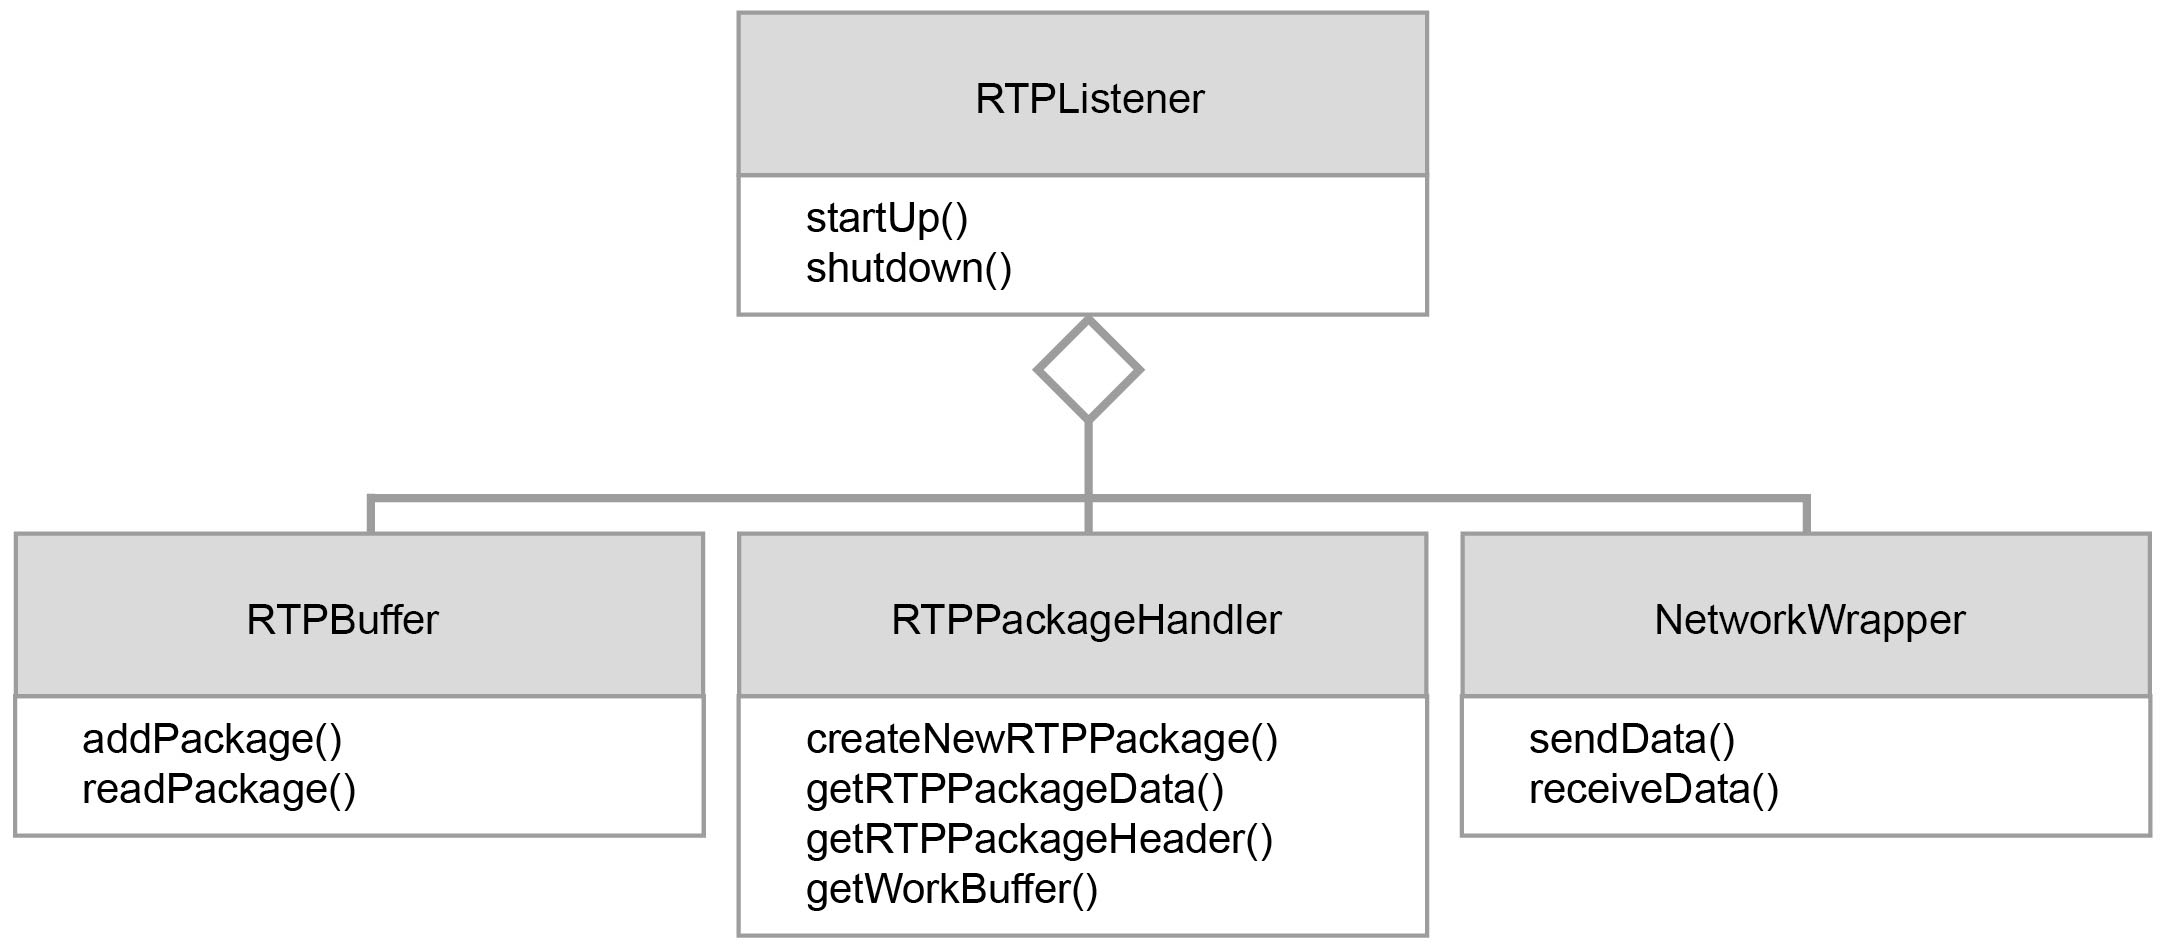
\includegraphics[width=1\textwidth]{../img/RTPListenerAdvanced}
\caption{Der gesamte Empfangsprozess in einem separaten Thread}
\label{Fig:RTPListenerAdvanced}
\end{figure}

Die Methode \texttt{startUp()} startet den \texttt{RTP"-Listener} in einem separaten Thread und \texttt{shut"-down()} beendet ihn wieder. Der Empfangsprozess besteht aus den Komponenten \texttt{RTP"-Buffer}, \texttt{RTP"-Package"-Handler} und dem \texttt{Network"-Wrapper}. Im Thread des \texttt{RTP"-Listeners} wird in einer Endlosschleife die blockierende Funktion \texttt{receive"-Data()} des \texttt{Network"-Wrappers} aufgerufen. Als Parameter wird der Funktion der Buffer des \texttt{RTP"-Package"-Handlers} übergeben. Hierfür wird die Funktion \texttt{getWork"-Buffer()} verwendet. Wenn ein Paket empfangen wurde, so kann mit Hilfe von \texttt{RTP"-Package"-Handler} der RTPHeader ausgelesen. Falls keine weitere Verarbeitung nötig ist, kann das Paket im \texttt{RTP"-Buffer} mit \texttt{add"-Package()} zwischengespeichert werden. Anschließend kann es mit \texttt{readPackage()} wieder ausgelesen werden. Das Auslesen des Paket erfolgt in der Regel vom Main-Thread, welches ohne Probleme möglich, da der \texttt{RTPBuffer} thread-safe ist.

\FloatBarrier

\section{Konkrete Softwarekomponenten}
\subsection{RTAudio}
\label{sec:RTAudio}
\subsection{Opus}
\section{Statistiken}
Ein weiteres Feature des OHMComm-Frameworks ist das Sammeln und Anzeigen von statistischen Daten. Die verschiedenen Statistiken wurden eingebaut, um die Performance einzelner Abschnitte der Verarbeitungskette zu messen, sowie die Richtigkeit der Handhabung von RTP-Paketen und frei gewählter Werte zu beweisen. Im Laufe des Programms werden eine Vielzahl an verschiedenen statistischen Daten gesammelt. Darunter fallen:
\begin{description}
\item[Audio-Daten:] Bei jedem Durchlauf der Verarbeitungskette werden Zähler für die Gesamtzahl der aufgenommenen sowie abgespielten Samples und Daten-Bytes erhöht.
\item[RTP-Daten:] Ebenso werden die Anzahl an versendeten und empfangenen RTP-Paketen, sowie die Größe deren Nutzdaten und der RTP-Header gezählt. Für das bestimmen der Quality of Service werden die Anzahl der verlorenen Pakete gezählt, sowie der maximale Füllstand des Jitter-Buffers gespeichert.
\item[Prozessor-Daten:] Wenn das messen der Prozessorlaufzeiten aktiviert ist, wird für jeden Audioprozessor in der Verarbeitungskette die Gesamtlaufzeit der beiden Methoden zum Bearbeiten der aufgenommenen oder abgespielten Daten gemessen.
\end{description}
Aus diesen gemessenen Werten werden beim Beenden des Frameworks verschiedene relevante Statistiken berechnet und ausgegeben. Die Ausgabe der Statistiken erfolgt immer über den Standardoutput (meist eine Konsole) sowie (falls vorher so konfiguriert) in eine Datei. Angezeigt werden die folgenden statistischen Werte:
\begin{itemize}
\item Die Gesamtzahl der aufgenommen und abgespielten Audiodaten (in Bytes) sowie Samples. Ebenso werden diese Werte durch die Gesamtlaufzeit der Kommunikation geteilt, um den Durchsatz der Soundkarte zu berechnen. An den Ergebnissen (vor allem an der Input- und Output-Samplerate) lässt sich erkennen, dass die Soundkarte sich nicht ganz an die vorher konfigurierte Samplerate hält, sondern leicht davon abweicht.
\item Die Gesamtzahl der gesendeten und empfangenen Daten (in Bytes) sowie Pakete. Wie auch im vorherigen Punkt sind hier die Durchsatz-Raten von größerer Bedeutung als die Gesamtzahlen. So wird hier der Datendurchsatz für die gesendeten und empfangene Pakete ausgerechnet, also die wirklich benötigte Bandbreite in beide Richtungen. Ebenso werden die Bandbreiten der reinen Audiodaten und der prozentuale Overhead der RTP-Header ausgegeben. Der Header-Overhead ist abhängig von der Größe der Daten in einem RTP-Paket und liegt meist unter 5\%.
\item Die Anzahl der verlorenen Pakete (also nicht empfangene Sequenznummern, siehe Abschnitt \ref{rtp}) sowie der maximale Füllstand der Jitter-Buffers. Anhand dieser Werte kann die Übertragungsqualität sowie die maximale Abspielverzögerung (der maximale \enquote{playout point}) abgelesen werden. Für beide Werte gilt, je kleiner der Wert, desto besser ist die Qualität der Übertragung.
\item Aus der Gesamtmenge an aufgenommenen/abgespielten Audiodaten und der Gesamtmenge an gesendeten/empfangen Audiodaten lässt sich die Kommpressions-/Dekompressionsrate berechnen, also wir stark ein verwendeter Audiocodec die Größe der Audiodaten komprimiert. Bei einer Kommunikation ohne zugeschalteten Audiocodec wird exakt die gleiche Anzahl an Bytes gesendet, die aufgenommen wird oder auch abgespielt, die empfangen wird, wodurch eine Kompression von 0\% angezeigt wird. Eine Verwendung des Opus-Codecs resultiert z.B. in einer Kompression von ca. 96\%, also werden nur 4\% der aufgenommen Audio-Bytes über das Netzwerk versendet und auch aus den empfangenen 4\% beim Entpacken wieder die volle Anzahl an Audiodaten wieder hergestellt. Daran kann man sehr gut die Bedeutung eines Audiocodecs für das Minimieren der benötigten Bandbreite erkennen.
\item Die Laufzeiten der verschiedenen Audioprozessoren. Wenn das Messen der Ausführungszeiten der Verarbeitungskette aktiviert wird, wird für jeden verwendeten Audioprozessor die Gesamtausführungszeiten der Methoden zum Bearbeiten des Audio-Inputs und -Outputs angezeigt. Auch hier wird zusätzlich der interessantere Wert der Ausführungszeit pro Aufruf ausgegeben, an dem die sog. algorithmische Verzögerung eines einzelnen Prozessors und der ganzen Verarbeitungskette abgelesen werden kann. Wenn die algorithmische Verzögerung der gesamten Prozessorkette zu groß wird, bekommt die Soundkarte nicht rechtzeitig neue Audiodaten und es wird ein hörbares Knacken ausgegeben.
\end{itemize}

\chapter{Implementierung}
In diesem Kapitel wird auf Implementierungsdetails des Entwurfs eingegangen. Hierbei ist zu beachten, dass aus Platzgründen der vorliegende Code eventuell in gekürzter oder geänderter Form dargestellt wird und unvollständig ist. Dennoch verdeutlichen die Codebeispiele die wesentlichsten Details der Implementierung und sind gemäß des Entwurfs umgesetzt.

\section{Verarbeitungskette}
Die Verarbeitungskette ist ein Teil des \texttt{AudioHandlers} und einer der wichtigen Komponenten des Frameworks. Sie ist die Schnittstelle, mit der anderen Klassen an der Audioverarbeitung teilnehmen können. Im folgenden Kapitel wird erörtert, wie diese implementiert wurde.

\subsection{Interface für Audioverarbeitungsklassen}
Alle Audioverarbeitungsklassen müssen die abstrakte Klasse \texttt{Audio"-Processor} implementieren, siehe Listening \ref{Code:AudioProcessor}.

\begin{lstlisting}[caption={Interface des AudioProcessors},label={Code:AudioProcessor}]
class AudioProcessor {
public:
	AudioProcessor(const std::string name);
	virtual unsigned int processInputData(void *inputBuffer, int inputBufferByteSize) = 0;
	virtual unsigned int processOutputData(void *outputBuffer,  int outputBufferByteSize) = 0;
}
\end{lstlisting}
Der Konstruktor in Zeile 4 erwartet als Parameter den Namen des Audioprozessors, damit dieser später eindeutig identifiziert werden kann. Die beiden Verarbeitungsmethoden in Zeile 5 und 6 sind virtuell, daher müssen alle Unterklassen diese implementieren. Diese Methoden stellen die Schnittstelle zur Audioverarbeitung dar und haben als Parameter jeweils den Buffer sowie die Buffergröße.

\subsection{An- und Abmeldeprozess im AudioHandler}
Listening \ref{Code:AudioHandlerAdd} zeigt die Schnittstelle zum An- und Abmelden von Audioprozessoren im \texttt{AudioHandlers} an. Die Methode \texttt{addProcessor()} fügt einen Audioprozessor in die Audioverarbeitungsliste ein, falls er noch nicht vorhanden ist, und \texttt{removeProcessor()} ist die entsprechende Löschmethode. Als Liste wird hier der Standardcontainer \texttt{std::vector} benutzt. Bei diesem werden neue Elemente am Ende der Liste eingefügt.

\begin{lstlisting}[caption={An- und Abmeldeprozess von Audioprozessoren im AudioHandler},label={Code:AudioHandlerAdd}]
bool AudioHandler::addProcessor(AudioProcessor *audioProcessor)
{
	if (hasAudioProcessor(audioProcessor) == false) {
		audioProcessors.push_back(std::unique_ptr<AudioProcessor>(audioProcessor));
		return true;
	}
	return false;
}

bool AudioHandler::removeAudioProcessor(AudioProcessor *audioProcessor) {
	for (size_t i = 0; i < audioProcessors.size(); i++)
	{
		if ((audioProcessors.at(i))->getName() == audioProcessor->getName()) {
			audioProcessors.erase(audioProcessors.begin() + i);
			return true;
		}	
	}
	return false;
}
\end{lstlisting}

\subsection{Verarbeitungsprozess}
Listening \ref{Code:AudioHandlerProcess} zeigt den Verarbeitungsprozess. Die Methode \texttt{processAudioInput()} wird vom AudioHandler aufgerufen, falls Daten vom Mikrofon zur Verarbeitung anliegen. Dort wird von jedem angemeldeten Audioprozessor die entsprechende \texttt{processInputData()} -Methode aufgerufen. Als Parameter werden die Daten des Mikrofons und deren Datengröße übergeben. Die Verarbeitungsreihenfolge entspricht der Anmeldereihenfolge. Die Verarbeitung im Buffer erfolgt in-place, daher auf den übergebenen Buffer. Falls ein Audioprozessor zu Beginn die Daten manipuliert, so sind diese Daten für alle nachfolgenden Prozessoren ebenfalls geändert. Im Umkehrschluss heißt dies, um wieder an die Ursprungsdaten zu gelangen, müssen die ausgeführten Änderungen in umgekehrte Reihenfolge rückgängig gemacht zu werden. \texttt{processAudioOutput()} wird aufgerufen, wenn die Soundkarte bereit ist Audiodaten abzuspielen. Hierzu werden von allen Audioprozessoren die \texttt{processOutputData()} - Methoden aufgerufen, jedoch mit umgekehrter Aufrufreihenfolge, siehe Zeile 13. Dadurch wird der Ursprungszustand der Audiodaten hergestellt und sind abspielbar.

\begin{lstlisting}[caption={Verarbeitungsprozess des AudioHandlers},label={Code:AudioHandlerProcess}]
void AudioHandler::processAudioInput(void *inputBuffer,  int inputBufferByteSize)
{
	unsigned int bufferSize = inputBufferByteSize;
	for (unsigned int i = 0; i < audioProcessors.size(); i++)
	{
		bufferSize = audioProcessors.at(i)->processInputData(inputBuffer, bufferSize);
	}
}

void AudioHandler::processAudioOutput(void *outputBuffer, int outputBufferByteSize)
{
	unsigned int bufferSize = outputBufferByteSize;
	for (unsigned int i = audioProcessors.size(); i > 0; i--)
	{
		bufferSize = audioProcessors.at(i-1)->processOutputData(outputBuffer, bufferSize);
	}
}
}\end{lstlisting}

\section{Factory-Klassen}
Die beiden Factory-Klassen \texttt{AudioHandlerFactory} und \texttt{AudioProcessorFac\-tory} sind vom Aufbau identisch, deshalb wird im folgenden nur die \texttt{AudioHandler\-Factory} erklärt. \texttt{AudioProcessorFactory} verhält sich analog dazu. Die Factory-Klassen haben die Aufgabe die Instantiierung in Methoden auszulagern, damit das Programmieren auf Schnittstellen gewährleistet wird. Methoden die Instantiierung übernehmen werden auch Fabrikmethoden genannt \cite{Goll2013}[S.243]. Listening \ref{Code:AudioHandlerFactory} zeigt die Fabrikmethode der \texttt{AudioHandlerFactory}. Als Parameter wird der Name der zu erzeugende Klasse entgegen genommen. Der Rückgabewert der Funktion entspricht den abstrakten und gemeinsamen Basistypen.

\begin{lstlisting}[caption={Fabrikmethode der AudioHandlerFactory},label={Code:AudioHandlerFactory}]
std::unique_ptr<AudioHandler> AudioHandlerFactory::getAudioHandler(std::string name) {
	if (name == RTAUDIO_WRAPPER)
	{
		std::unique_ptr<RtAudioWrapper> rtaudiowrapper(new RtAudioWrapper);
		return std::move(rtaudiowrapper);
	}
	throw std::invalid_argument("No AudioHandler for this name!");
}
\end{lstlisting}

\section{RTPListener}
\texttt{RTPListener} ermöglicht das asynchrone Empfangen von Paketen durch das Erstellen eines eignen Threads. Die wichtigsten Methoden der Klasse sind im Listening \ref{Code:RTPListener} dargestellt. Die \texttt{startUp()}-Methode startet den Thread und \texttt{shutdown()} beendet ihn wieder. Sobald der Thread startet wird \texttt{runThread()} aufgerufen. Tatsächlich ist diese Methode komplexer, wurde jedoch für das Beispiel auf das wesentliche gekürzt. In der Schleife wird die blockierende \texttt{receiveData()}-Funktion aufgerufen. Übertragene Packete werden im Jitter-Buffer zwischengespeichert, siehe Zeile 14. Die empfangenen Pakete können anschließend aus dem Jitter-Buffer von anderen Threads ausgelesen werden. Der \texttt{RTPListener} wartet anschließend wieder auf neue ankommende Pakete.

\begin{lstlisting}[caption={Die wichtigsten Methoden des RTPListeners},label={Code:RTPListener}]
void RTPListener::startUp()
{
    threadRunning = true;
    receiveThread = std::thread(&RTPListener::runThread, this);
}

void RTPListener::shutdown(){
	threadRunning = false;
}

void RTPListener::runThread() {
	while(threadRunning) {
		int receivedSize = this->wrapper->receiveData(rtpHandler.getWorkBuffer(), rtpHandler.getMaximumPackageSize());
		auto result = buffer->addPackage(rtpHandler, receivedSize - RTP_HEADER_MIN_SIZE);
	}
}
\end{lstlisting}

\section{RtAudio}

Der \textbf{RtAudioWrapper} bietet drei Modi zur Audiokommunikation, diese sind \textit{RecordingMode}, \textit{PlaybackMode} und \textit{DuplexMode}. Bei den ersten beiden Modi wird entweder nur der Input- oder der Output-Stream übergeben um nur Sound aufzunehmen oder abzuspielen. Dagegen benutzt der letzte Modus(DuplexMode) den input und output Stream um ein simultanes aufnehmen und abspielen von Audio Daten zu ermöglichen.

Die RtAudio-API wird mittels eines Objekts, dessen Namen auf rtaudio definiert wurde gesteuert.

\begin{lstlisting}[caption={RtAudio Objekt und StreamParameter},label={Code:RtAudio Objekt}]
RtAudio rtaudio;
RtAudio::StreamParameters input, output;
\end{lstlisting}

Um den \textit{Duplex Modus} zu starten wird zuerst per Flag (\texttt{flagPrepare}) geprüft ob die \texttt{prepare()}-Methode von RtAudioWrapper bereits ausgeführt worden ist -- welche überprüft ob die Output und Input Stream Parameter konfiguriert sind -- und ob alle AudioProzessoren mittels der \texttt{prepare()}-Methode des AudioHandler ihre Unterstützten Parameter gemeldet haben und sich auf einen gleichen Parametersatz einigen konnten. Wenn dies nicht der Fall ist, wird ein Fehler ausgegeben, mit dem Hinweis, dass die AudioProzessoren zuerst konfiguriert werden müssen, bevor der RtAudio Stream gestartet werden kann.

Dem \texttt{rtaudio}-Objekt werden per \texttt{openStream()}-Methode die benötigten Parameter mitgeteilt, welche folgenden Inhalt haben:

\begin{description}
\item[output] Der Output Stream Parameter, welcher die \texttt{deviceID}, also die ID des Hardware Geräts, welches die Audiosignale ausgeben soll und die Anzahl der zu benutzenden \textit{Channels} enthält. Diese sind entweder per \texttt{setDefaultAudio\-Config()}-Methode des RtAudioWrapper oder per \textit{FileConfiguration}, \textit{InteractiveConfiguration} oder \textit{ParameterConfiguration} vorher festgelegt worden.
\item [input] Der Input Parameter welcher die \texttt{deviceID} des Audiogeräts, welches die Audiosignale aufnimmt, und die Anzahl der aufzunehmenden \textit{Channels} enthält. Dieser ist ebenfalls bereits mittels einer der verschiedenen Konfigurationsmodi konfiguriert worden.
\item [audioConfiguration.audioFormatFlag] : Das Audioformat-Flag, welches das \textit{Audioformat} definiert(z.B. SINT16 oder FLOAT32), welches durch den AudioHandler durch Abfragen der AudioProzessoren ausgehandelt wurde.
\item [audioConfiguration.sampleRate] Die \textit{Sample Rate}, die vom AudioHandler durch Abfragen der AudioProzessoren ausgehandelt wurde.
\item [audioConfiguration.framesPerPackage] Die Anzahl der \textit{Frames} per Package, also die Größe des Audiobuffers. Diese Größe wurde auch vom AudioHandler durch Abfragen der AudioProzessoren ausgehandelt
\item [RtAudioWrapper::callbackHelper] Die \textit{Callback-Methode}, welche von der RtAudio-API aufgerufen wird, wenn Audiodaten vorhanden sind.
\item [this] Eine Referenz auf das eigene \textit{Callback-Objekt}, um innerhalb der Callback-Methode auf benötigte Informationen zuzugreifen.
\end{description}

Anschließend wird die RtAudio-API mittels \texttt{startStream()} gestartet.

\begin{lstlisting}[caption={Start des Duplex Mode im RtAudioWrapper},label={Code:RtAudio DuplexMode}]
void RtAudioWrapper::startDuplexMode()
{
 if (this->flagPrepared)
 {
  this->rtaudio.openStream(&output, &input, audioConfiguration.audioFormatFlag,   audioConfiguration.sampleRate, &audioConfiguration.framesPerPackage, &RtAudioWrapper::callbackHelper, this);
  this->rtaudio.startStream();
 }
}
\end{lstlisting}

Der \texttt{callbackHelper()} erstellt daraufhin ein \texttt{RtAudioWrapper}-Objekt und ruft dessen \texttt{callback()}-Methode auf. Diese Aufteilung wurde gewählt da hierdurch besser ersichtlich ist wo es sich um \textit{Eingabedaten}(von der RtAudio-API \texttt{callbackHelper()}-Methode) und wo um \textit{Ausgabedaten}(zu den AudioProzessoren \texttt{callback()}-Methode) handelt.

\begin{lstlisting}[caption={\texttt{callbackHelper()}-Methode im RtAudioWrapper},label={Code:RtAudio CallbackHelper}]
auto RtAudioWrapper::callbackHelper(void *outputBuffer, void *inputBuffer, unsigned int nBufferFrames, double streamTime, RtAudioStreamStatus status, void *rtAudioWrapperObject) -> int
{
 RtAudioWrapper *rtAudioWrapper = static_cast <RtAudioWrapper*> (rtAudioWrapperObject);
 return rtAudioWrapper->callback(outputBuffer, inputBuffer, nBufferFrames, streamTime, status, nullptr);
}
\end{lstlisting}

Die \texttt{callback()}-Methode des RtAudioWrapper ruft die Methoden \texttt{processAudio\-Input()} und \texttt{processAudioOutput()} auf welche die einzelnen Prozessoren durchläuft und folgende Parameter enthält :
\begin{description}
\item[inputBuffer] Pointer auf den Speicherbereich der die input Audio Daten enthält.
\item[outputBuffer] Pointer auf den Speicherbereich der die output Audio Daten enthält.
\item[inputBufferByteSize] Größe der Daten die im inputBuffer vorhanden sind.
\item[outputBufferByteSize] Größe der Daten die im outputBuffer vorhanden sind.
\item[streamData] Struct welcher zusätzliche Informationen zu den Daten im Audio Buffer enthält, wie die Anzahl der Frames im Buffer(\texttt{nBufferFrames}), die Aktuelle Zeit des Streams(\texttt{streamTime}) und die Maximale Anzahl der Daten welche in den Buffer geschrieben werden könne(\texttt{maxBufferSize}).
\end{description}

\begin{lstlisting}[caption={callback Methode im RtAudioWrapper},label={Code:RtAudio Callback}]
auto RtAudioWrapper::callback(void *outputBuffer, void *inputBuffer, unsigned int nBufferFrames, double streamTime, RtAudioStreamStatus status, void *rtAudioWrapperObject) -> int
{
 (...)
 this->processAudioInput(inputBuffer, inputBufferByteSize, streamData);
 (...)
 this->processAudioOutput(outputBuffer, outputBufferByteSize, streamData);
}
\end{lstlisting}

\section{Opus}

Der \textbf{Opus-Codec}, welcher zum \textit{Encoden} und \textit{Decoden} der Audiodaten benutzt wird wurde als \textit{Prozessor} in OHMComm eingebunden.

Der \textit{Konstruktor} des Opus-Prozessors erstellt bei der Instanziierung jeweils ein Encoder- und Decoder-Objekt. Außerdem wird ihm ein Name gegeben und der Opus-Application-Type (siehe \ref{Opus Application Modi}) wird gewählt.

\begin{lstlisting}[caption={Instanziierung des Opus Prozessors},label={Code:Opus Instanziierung}]
ProcessorOpus::ProcessorOpus(const std::string name, int opusApplication) : AudioProcessor(name), OpusEncoderObject(nullptr), OpusDecoderObject(nullptr)
{
    this->OpusApplication = opusApplication;
}
\end{lstlisting}

Anschließend werden die Encoder- und Decoder-Objekte in der \texttt{configure()}-Methode konfiguriert. Dies geschieht mit dem Aufruf der \texttt{opus\_encoder\_create()} bzw. \texttt{opus\_decoder\_create()}-Methoden. Die Parameter hierbei sind:
\begin{description}
\item[audioConfig.sampleRate] Die \textit{Sample Rate} der Audio Daten. Welche einen der von Opus unterstützen Werte haben muss siehe \ref{Opus Sample Rate}.
\item[audioConfig.inputDeviceChannels] Die Anzahl der input \textit{Channels}.
\item[audioConfig.outputDeviceChannels] Die Anzahl der output \textit{Channels}.
\item[OpusApplication] Der \textit{Opus-Application-Type} siehe \ref{Opus Application Modi}.
\item[ErrorCode] Eine Variable welche im Fehlerfall den \textit{Error Code} zur Fehlerbehandlung enthält.
\end{description}

\begin{lstlisting}[caption={Konfiguration der Opus Encoder und Decoder-Objekte},label={Code:Opus Konfiguration}]
bool ProcessorOpus::configure(const AudioConfiguration& audioConfig, const std::shared_ptr<ConfigurationMode> configMode)
{
	(...)
	OpusEncoderObject = opus_encoder_create(audioConfig.sampleRate, audioConfig.inputDeviceChannels, OpusApplication, &ErrorCode);
	OpusDecoderObject = opus_decoder_create(audioConfig.sampleRate, audioConfig.outputDeviceChannels, &ErrorCode);
	(...)
}
\end{lstlisting}

Das \textit{Encodieren} der Audiodaten geschieht in der \texttt{processInputData()}-Methode des Opus-Prozessors. Zu Beginn wird die Variable \texttt{lengthEncodedPacketIn\-Bytes} deklariert in der die Größe der Audiodaten nach ihrer Encodierung gespeichert wird. Anschließend wir geprüft ob Daten im 16-bit Signed-Integer-Format oder im 32-bit Float-Format vorliegen.
Abhängig davon wir die entsprechende \texttt{opus\_encode()}-Methode aufgerufen, welche folgende Parameter benötigt:

\begin{description}
\item[OpusEncoderObject] Das bei der Instanziierung erzeugte und in der \texttt{configure()}-Methode konfigurierte Opus \textit{Encoder Objekt}.
\item[inputBuffer] Der ins 16-bit Signed-Integer oder 32-bit Float Format gecastete \textit{InputBuffer} Pointer welcher die Input Audio Daten der Soundkarte enthält.
\item[userData->nBufferFrames] Die Anzahl der \textit{Samples}(per Channel) welche sich im InputBuffer befinden. Da Opus Audioframegrößen von 2.5ms bis 60ms unterstützt (siehe \ref{Opus Audioframe}), muss die Anzahl der Samples auch in diesem Bereich liegen. Bei 48kHz Sample Rate und einer Audioframegröße von 20ms also 960 Samples pro Channel.
\item[inputBuffer] Char-Pointer der Anzeigt wohin die Encodierten Audio Daten geschrieben werden sollen. Da wir auf dem \textit{InputBuffer} Arbeiten und keinen extra Speicherplatz für Encodierte Daten haben, ist dies der selbe Speicherbereich aus dem wir die Daten gelesen haben.
\item[userData->maxBufferSize] Maximal Größe des Speicherbereichs wohin die Encodierten Daten geschrieben werden.
\end{description}

Als Rückgabewert geben wir die neue Größe des \texttt{inputBuffers} weiter. 


\begin{lstlisting}[caption={Encodieren von Audio Daten mittels Opus},label={Code:Opus Encodieren}]
unsigned int ProcessorOpus::processInputData(void *inputBuffer, const unsigned int inputBufferByteSize, StreamData *userData)
{
    unsigned int lengthEncodedPacketInBytes = 0;
    if (rtaudioFormat == AudioConfiguration::AUDIO_FORMAT_SINT16)
    {
        lengthEncodedPacketInBytes = opus_encode(OpusEncoderObject, (opus_int16 *)inputBuffer, userData->nBufferFrames, (unsigned char *)inputBuffer, userData->maxBufferSize);
        return lengthEncodedPacketInBytes;
    }
    else if (rtaudioFormat == AudioConfiguration::AUDIO_FORMAT_FLOAT32)
    {
        lengthEncodedPacketInBytes = opus_encode_float(OpusEncoderObject, (const float *)inputBuffer, userData->nBufferFrames, (unsigned char *)inputBuffer, userData->maxBufferSize);
        return lengthEncodedPacketInBytes;
    }
}
\end{lstlisting}

Das \textit{Decodieren} geschieht auf ähnliche Weise wie das Encodieren der Audio Daten innerhalb der \texttt{processOutputData()}-Methode.
Zuerst wird eine Variable angelegt, in der die Anzahl der decodierten Samples gespeichert wird(\texttt{numberOfDecoded\-Samples}), welche von der \texttt{opus\_decode()}-Methode als Rückgabewert zurückgeliefert wird. Es wird wieder geprüft, ob die Daten im 16-bit Signed-Integer-Format oder im 32-bit Float-Format decodiert werden sollen. Anschließend wird die \texttt{opus\_decode()}-Methode mit folgenden Parametern aufgerufen:

\begin{description}
\item[OpusDecoderObject] Das bei der Instanziierung erzeugte und in der \texttt{configure()}-Methode konfigurierte Opus \textit{Decoder Objekt}.
\item[outputBuffer] Char-Pointer auf die Encodierten Audio Daten.
\item[outputBufferByteSize] Größe des OutputBuffers.
\item[outputBuffer] Pointer wohin die Decodierten Audio Daten geschrieben werden sollen entweder im Signed Integer 16 oder Float 32 Format.
\item[userData->maxBufferSize] Maximal Anzahl der \textit{Samples} welche in den Speicherbereich der Decodierten Daten geschrieben werden können.
\item[0] Möglicher Platz für ein \textit{Flag} welches Anzeigt ob in-band forward error correction Daten vorhanden sind, was nicht der Fall ist.
\end{description}

Da wir als \textit{Rückgabewert} von \texttt{opus\_decode()} die Anzahl der decodierten Samples bekommen, die Prozessoren aber als Rückgabewert die Größe des OutputBuffers zurückgeben sollen, muss diese noch Mittels der Anzahl der decodierten Samples multipliziert mit der Größe des gewünschten Formates multipliziert mit der Anzahl der Channels \texttt{(numberOfDecodedSamples * sizeof(opus\_int16) * outputDeviceChannels)} berechnet werden.

\begin{lstlisting}[caption={Decodieren von Audio Daten mittels Opus},label={Code:Opus Decodieren}]
unsigned int ProcessorOpus::processOutputData(void *outputBuffer, const unsigned int outputBufferByteSize, StreamData *userData)
{
    unsigned int numberOfDecodedSamples = 0;
    if (rtaudioFormat == AudioConfiguration::AUDIO_FORMAT_SINT16)
    {
        numberOfDecodedSamples = opus_decode(OpusDecoderObject, (unsigned char *)outputBuffer, outputBufferByteSize, (opus_int16 *)outputBuffer, userData->maxBufferSize, 0);
        userData->nBufferFrames = numberOfDecodedSamples;
        const unsigned int outputBufferInBytes = (numberOfDecodedSamples * sizeof(opus_int16) * outputDeviceChannels);
        return outputBufferInBytes;
    }
    else if (rtaudioFormat == AudioConfiguration::AUDIO_FORMAT_FLOAT32)
    {
        numberOfDecodedSamples = opus_decode_float(OpusDecoderObject, (const unsigned char *)outputBuffer, outputBufferByteSize, (float *)outputBuffer, userData->maxBufferSize, 0);
        userData->nBufferFrames = numberOfDecodedSamples;
        const unsigned int outputBufferInBytes = (numberOfDecodedSamples * sizeof(float) * outputDeviceChannels);
        return outputBufferInBytes;
    }
}
\end{lstlisting}

\FloatBarrier
\section{Passive Konfiguration}
\label{passiveConfiguration}
Die passive Konfiguration aus Abschnitt \ref{configurationUsages} wird mithilfe von \textbf{Application-defined} RTCP-Paketen aus Abschnitt \ref{rtcp} umgesetzt. Hierfür wird für die Konfiguration einer Sitzung der Klient \textbf{A} mit der Option \enquote{Konfigurationsanfrage aktivieren} (oder dem Parameter \texttt{--wait-for-passive}) gestartet, um eine Anfrage einer passiven Konfiguration zu ermöglichen. Klient \textbf{B} wird mit dem Parameter \texttt{--passive} ausgeführt. Klient \textbf{A} konfiguriert das OHMComm-Framework, startet jedoch noch keine Kommunikation, sondern nur den RTCP-Thread und wartet dort auf eine Anfrage für eine passive Konfiguration. Klient \textbf{B} sendet eine RTCP Application-defined Nachricht an \textbf{A}, die die Anfrage einer passiven Konfiguration darstellt. Daraufhin antwortet \textbf{A} mit einem weiteren RTCP-Paket, das die Werte der passiven Konfiguration (Abtastrate, Audioformat, Audiocodecs, Anzahl der Kanäle sowie die Puffergröße) beinhaltet. Dieses Paket wird von \textbf{B} empfangen und die Konfiguration ausgelesen. Daraufhin können beide Seiten das Übertragen von Audiodaten beginnen. Durch die Übertragung aller relevanten Informationen (Einstellungen der Audiobibliothek sowie die verwendeten Audiocodecs) wird garantiert, dass die gesendeten Daten von der anderen Instanz auch verstanden und verwendet werden können. Um die passive Konfiguration zu starten, wird für den Klienten \textbf{B} nur die IP-Adresse und der Port des Klienten \textbf{A} benötigt, wohingegen \textbf{A} komplett wie bereits beschrieben konfiguriert werden kann. Der Ablauf einer passiven Konfiguration ist schematisch in Listing \ref{lst:passiveConfiguration} dargestellt:
\newline
\begin{figure}[htp]
\centering
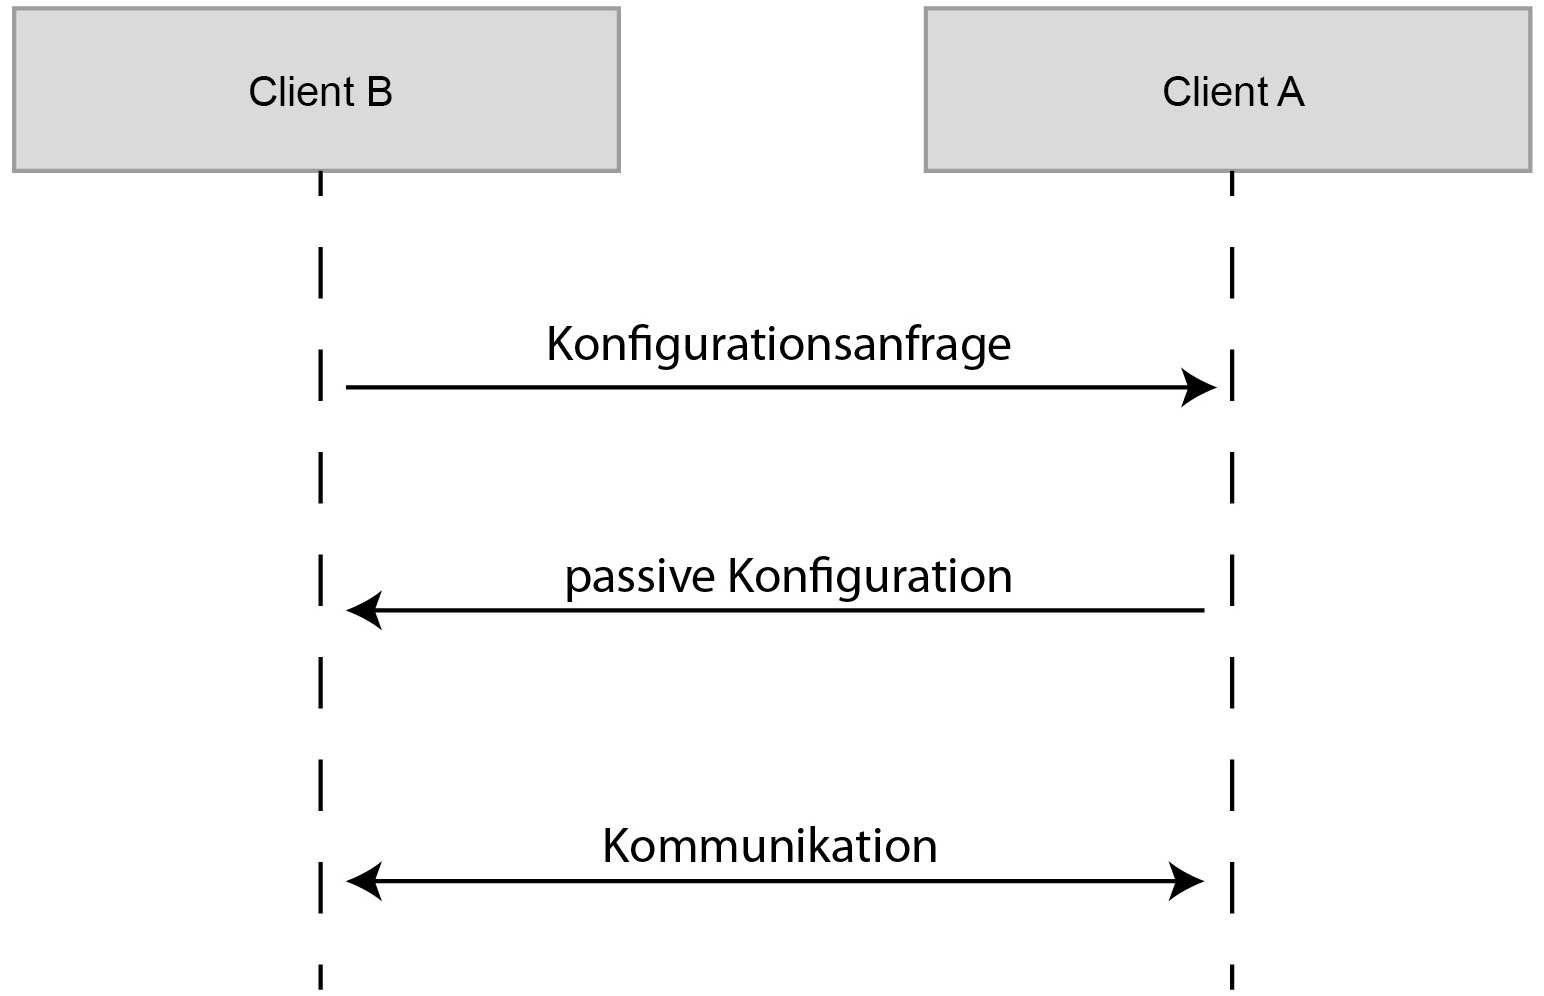
\includegraphics[width=.75\textwidth]{../img/passiveConfiguration}
\caption{Ablauf der passiven Konfiguration}
\label{lst:passiveConfiguration}
\end{figure}

\FloatBarrier
%\begin{lstlisting}[keepspaces=true,numbers=none,label=lst:passiveConfiguration,caption=Ablauf der passiven Konfiguration,xleftmargin=.2\textwidth, xrightmargin=.2\textwidth]
%Client B                            Client A
%  |                                       |
%  |         Konfigurationsanfrage         |
%  |-------------------------------------->|
%  |                                       |
%  |         passive Konfiguration         |
%  |<--------------------------------------|
%  |                                       |
%  |             Kommunikation             |
%  |<------------------------------------->|
%\end{lstlisting}
\chapter{Prototypische Voice-over-IP Konsolenanwendungen}
\label{prototypProgram}
\section{Ziel der Anwendung}
\section{Verwendung der Schnittstelle des Frameworks}
Das OHMComm-Framework bietet eine sehr übersichtliche Schnittstelle, die verwendet werden muss, um das Framework in eine Anwendung einzubinden. Diese Schnittstelle ist eine Instanz der Klasse \texttt{OHMComm}, über die das gesamte Framework gesteuert werden kann. Um diese Schnittstelle nun verwenden zu können, muss ein \texttt{OHMComm}-Objekt erstellt werden. Dafür muss vorher eine Konfiguration als Instanz einer der \texttt{ConfigurationMode}-Kindklassen erstellt werden. Diese wird dem Konstruktor \texttt{OHMComm(ConfigurationMode*)} übergeben und das Framework kann verwendet werden. Daraufhin wird mit der Methode \texttt{isConfigurationDone\allowbreak{}(bool)} überprüft, ob die Konfiguration abgeschlossen ist, die über den Flag-Parameter gestartet werden kann, falls dies nicht so ist. Die restlichen Funktionalitäten werden danach automatisch, je nach übergebener Konfiguration, aktiviert und eingestellt. Damit ist das Framework vollständig eingestellt und die Kommunikation kann mit einem Methodenaufruf auf \texttt{startAudioThreads()} gestartet werden. Dieser Aufruf ist nicht blockierend, so dass der aufrufende Thread weitere Aktivitäten ausführen kann. Solang die Kommunikation läuft, gibt die Methode \texttt{isRunning()} \texttt{true} zurück. Beendet wird das Framework über die Methode \texttt{stopAudioThreads()}. Einen Beispielcode über die Verwendung des Frameworks liefert die prototypische Anwendung in der Datei \texttt{OHMCommStandalone.cpp}.
\section{Steuerung}
Die \texttt{main()}-Funktion aus \texttt{OHMCommStandalone.cpp} implementiert vier der fünf verfügbaren Konfigurationsmodi (siehe Abschnitt \ref{configurationUsages}). Die prototypische Konsolenanwendung kann also auf vier verschiedene Arten konfiguriert werden:
Wird das Programm ohne Kommandozeilenargumenten gestartet, wird die interaktive Konfiguration verwendet, bei der die benötigten Einstellungen nacheinander auf der Konsole mit möglichen Werten ausgegeben werden und der Benutzer durch Texteingabe die Einstellungen setzen muss.  Wird das Programm mit einem einzelnen Dateipfad als Parameter gestartet, werden die Einstellungen aus der übergebenen Datei geladen. Wenn das Kommandozeilenargument \texttt{-P} oder \texttt{--passive} gesetzt ist, wird die zusätzlich als Argument mit übergebene Netzwerkkonfiguration dazu verwendet, um eine Anfrage für eine passive Konfiguration an diese Adresse zu senden (siehe Abschnitt \ref{passiveConfiguration}). Der letzte implementierte Konfigurationsmodus ist die Parameterkonfiguration, bei der alle Einstellungen als Kommandozeilenargumente an den Programmaufruf angehängt werden, wobei mit \texttt{-h} oder \texttt{--help} eine Übersicht über alle möglichen Einstellungen ausgegeben werden kann.
\section{Anwendungen ordnungsgemäß beenden}
Ein größeres Problem bei der Umsetzung der prototypischen Konsolenanwendung ist es gewesen, die Anwendung ordnungsgemäß zu beenden. Besonders problematisch wird es, da die Anwendung aus verschiedenen Threads besteht, die alle beendet werden müssen, sowie die Kommunikation selber aus verschiedenen Threads heraus beendet werden kann. So müssen folgende Threads beendet werden: Der Thread der Verarbeitungskette, der von der Audioschnittstelle heraus gestartet wird, der RTPListener-Thread und der RTCP-Thread, die beide vom \texttt{OHMComm}-Objekt erzeugt werden. Ebenso muss der \texttt{NetworkWrapper} geschlossen werden, da dieser auch verbindungsorientiert (z.B. mit TCP) implementiert werden kann. Beendet werden kann das Framework an folgenden Stellen: von Extern (z.B. der verwendenden Anwendung) und durch den RTCP-Thread (beim Empfangen eines \texttt{BYE}-Pakets). Daher muss dafür gesorgt werden, dass sowohl der aufrufende Code als auch der RTCP-Thread Zugriff auf die \texttt{stopAudioThreads()}-Methode des \texttt{OHMComm}-Objekts haben. Dafür wird dem RTCP-Thread ein Funktionsobjekt mitgegeben, das die \texttt{stopAudioThreads()}-Methode aufruft, die dafür sorgt, dass alle vom Framework erstellten Threads und Resource-Handler ordnungsgemäß beendet und geschlossen werden.
\\
Somit kann die Kommunikation im OMHComm-Framework durch den Aufruf der \texttt{stopAudioThreads()}-Methode aus allen Stellen, die Zugriff darauf haben ordnungsgemäß und vollständig beendet werden. Jedoch wird die Kommunikation im Framework durch einen nicht blockierenden Methodenaufruf auf \texttt{startAudio\-Threads()} gestartet, damit der aufrufende Thread weitere Tätigkeiten ausführen kann. Da aber ein Programm automatisch beendet wird, wenn die \texttt{main()}-Funktion ihr Ende erreicht, muss für die prototypische Konsolenanwendung der Haupt-Thread nach dem Start der Kommunikation solange schlafen gelegt werden, bis die Kommunikation beendet wird. Dafür wird in der \texttt{main()}-Funktion blockierend auf eine Benutzereingabe gewartet und nach dieser Eingabe die Kommunikation und schließlich das Programm beendet. Wird jedoch die Kommunikation über einen anderen Weg (z.B. durch das Empfangen eines RTCP \texttt{BYE}-Pakets) beendet, wartet der Haupt-Thread weiterhin auf eine Benutzereingabe und somit läuft das Konsolenprogramm weiter. Deshalb muss derzeit die Konsolenanwendung immer mit einer Benutzereingabe (beliebige Zeichen, die mit einem \enquote{Enter} abgesendet werden) beendet werden.
\chapter{Fazit und Ausblick}
\section{Projektergebnis}
TODO: Evtl auch Vergleich mit Zielen/Aufgabenstellung
\section{Anwendungsmöglichkeiten}
Das OHMComm Framework kann als fertige plattformunabhängige Bibliothek für VoIP-Kommunikation in anderen Programme eingebaut werden. Dafür wird ein \texttt{OHMComm}-Objekt erstellt, konfiguriert (bevorzugt über die \texttt{LibraryConfiguration}) und die Kommunikation gestartet. Da die komplette Aktivität des Frameworks in anderen Threads (für Audioverarbeitung, Empfangen,, RTCP, ...) abläuft, wird der aufrufende Thread nicht blockiert und die Kommunikation kann von dem verwendenden Programm wieder beendet werden. Da OHMComm alle verwendeten Bibliotheken mitliefert und eine kleine und wohldefinierte Schnittstelle bietet, lässt es sich sehr einfach in andere Programme einbauen.
Ein Beispiel der Anwendbarkeit zeigt die in Kapitel \ref{prototypProgram} beschriebene prototypische Konsolenanwendung, die z.B. verwendet werden kann, um auf die Schnelle eine Audioübertragung zwischen zwei Geräten aufzubauen. Anhand dieser Beispielanwendung lassen sich sehr einfach die verschiedenen Konfigurationsmodi und Einstellungsmöglichkeiten ausprobieren. Der Code dazu (bestehend aus der Datei \texttt{OHMCommStandalone.cpp}) zeigt ein kurzes und vollständiges Beispiel, wie das Framework richtig eingebunden werden kann.
\section{Erweiterungsmöglichkeiten}
Aufgrund des modularen Aufbaus des kompletten Frameworks, lässt es sich sehr einfach erweitern. Vorgesehene Erweiterungen für das Framework gliedern sich in die folgenden Kategorien:
\begin{description}
\item[Parameter:] Alle existierenden Parameter können -- soweit einmal registriert -- von allen Audioprozessoren verwendet werden. Ebenso ist es sehr einfach, neue Parameter zu registrieren, die bei der Konfiguration des Frameworks automatisch beachtet und mit Werten versehen werden.
\item[Audioschnittstellen:] Derzeit wird als einzige Schnittstelle zur Audiohardware die Bibliothek RTAudio verwendet. Jedoch kann die Audiobibliothek einfach ausgetauscht werden, indem eine neue Kindklasse von \texttt{AudioHandler} erstellt und zur \texttt{AudioHandlerFactory} hinzugefügt wird, die auf einer anderen Audiobibliothek aufbaut. So könnte z.B. PortAudio, eine plattformunabhängige C-Audioschnittstelle, angebunden werden.
\item[Audioprozessoren:] In die Verarbeitungskette (siehe Abschnitt \ref{processingChain}) können beliebige neue Prozessoren für Audiodaten hinzugefügt werden. Dafür muss nur die neu erstellte Kindklasse von \texttt{AudioProcessor} in \texttt{AudioProcessorFactory} registriert werden und beim Start der Anwendung ausgewählt werden. Ebenso können -- wie bereits erwähnt -- neue Parameter für die Konfiguration der neuen Audioprozessoren registriert werden.
\item[Netzwerkschnittstellen:] Auch neue Schnittstellen für Netzwerkprotokolle, wie TCP, lassen sich durch Erstellen neuer Kindklassen von \texttt{NetworkWrapper} und Ersetzen der Aufrufe von \texttt{UDPWrapper} hinzufügen.
\end{description}
Derzeit sind Erweiterungen zu dem bestehenden Framework in Planung oder bereits in Entwicklung, wie die Konfiguration über das Session Initiation Protocol (SIP), sowie den Audiocodecs G.711 A-law und $\mu$-law, den Standardformaten der digitalen Telefonie.
\\
Im Allgemeinen können in die bestehende Architektur eine Vielzahl an zusätzlichen Funktionalitäten fest oder auch optional hinzugefügt werden. So z.B. weitere Audiocodecs, Hochpass- oder Tiefpassfilter zum Herausfiltern von Rauschen oder Hintergrundgeräuschen, Verstärker für die Lautstärke des abgespielten Signals, Prozessoren, die die Audiokonversation mitschneiden und viele mehr.


\bibliographystyle{apalike} % Literaturverzeichnis
\begin{btSect}{./sources/literatur} % mit bibtopic Quellen trennen
\section*{Literaturverzeichnis}
\btPrintCited
\end{btSect}
\begin{btSect}{./sources/online}
\section*{Online-Quellen}
\btPrintCited
\end{btSect}

\end{document}
